%%%%%%%%%%%%%%%%%%%%%%%%%%%%%%%%%%%%%%%%%%%%%%%%%%%%%%%%%%%%%%%%%%%%%%%%%%%%%%%%
%2345678901234567890123456789012345678901234567890123456789012345678901234567890
%        1         2         3         4         5         6         7         8

\documentclass[letterpaper, 10 pt, conference]{ieeeconf}  % Comment this line out if you need a4paper



%\documentclass[a4paper, 10pt, conference]{ieeeconf}      % Use this line for a4 paper

\IEEEoverridecommandlockouts                              % This command is only needed if 
                                                          % you want to use the \thanks command

\overrideIEEEmargins                                      % Needed to meet printer requirements.

%In case you encounter the following error:
%Error 1010 The PDF file may be corrupt (unable to open PDF file) OR
%Error 1000 An error occurred while parsing a contents stream. Unable to analyze the PDF file.
%This is a known problem with pdfLaTeX conversion filter. The file cannot be opened with acrobat reader
%Please use one of the alternatives below to circumvent this error by uncommenting one or the other
%\pdfobjcompresslevel=0
%\pdfminorversion=4

% See the \addtolength command later in the file to balance the column lengths
% on the last page of the document

% The following packages can be found on http:\\www.ctan.org
%\usepackage{graphics} % for pdf, bitmapped graphics files
%\usepackage{epsfig} % for postscript graphics files
%\usepackage{mathptmx} % assumes new font selection scheme installed
%\usepackage{times} % assumes new font selection scheme installed
\usepackage{amsmath} % assumes amsmath package installed
\usepackage{amssymb}  % assumes amsmath package installed
\usepackage{hyperref}


 \usepackage{easyReview}
 


\title{\LARGE \bf
Matrix Multiplication-Driven Repulsive Fields for Manipulator Kinematic Obstacle Avoidance
}


\author{
	Jakob Baumgartner$^{1}$ and Gregor Klančar$^{2}$% <-this % stops a space
%\thanks{*This work was not supported by any organization}% <-this % stops a space
%\thanks{$^{1}$Albert Author is with Faculty of Electrical Engineering, Mathematics and Computer Science,
%        University of Twente, 7500 AE Enschede, The Netherlands
%        {\tt\small albert.author@papercept.net}}%
%\thanks{$^{2}$Bernard D. Researcheris with the Department of Electrical Engineering, Wright State University,
%        Dayton, OH 45435, USA
%        {\tt\small b.d.researcher@ieee.org}}%
}


\begin{document}



\maketitle
\thispagestyle{empty}
\pagestyle{empty}


%%%%%%%%%%%%%%%%%%%%%%%%%%%%%%%%%%%%%%%%%%%%%%%%%%%%%%%%%%%%%%%%%%%%%%%%%%%%%%%%
\begin{abstract}



\end{abstract}

\add{ADD}


%%%%%%%%%%%%%%%%%%%%%%%%%%%%%%%%%%%%%%%%%%%%%%%%%%%%%%%%%%%%%%%%%%%%%%%%%%%%%%%%
\section{INTRODUCTION}

%The robots environment is modelled by discrete voxels. As the robots environment can dynamically change, we propose a method that looks at the surrounding space of the robot and calculates these direction away from all the surrounding obstacles in real time. We only look in a predefined area / perimeter arround the robot.  
%
%In 3D computer graphics, a voxel represents a value on a regular grid in three-dimensional space. Each of the voxels holds the probability value of its occupation. In case of voxel being empty it holds the value of 0, if the voxel is occupied it holds the value of non-zero, depending on our assurance of it being occupied. If it is definitly occupied it holds the value of 1. 

%Motion planning involves finding paths for manipulators through joint configurations from an initial to a goal position, respecting constraints and optimization criteria due to redundant degrees of freedom (DOF)~\cite{siciliano1990kinematic}. This redundancy allows for diverse configurations, optimizing secondary tasks like avoiding singularities and obstacles while maintaining the primary goal of reaching the End Effector (EE) target~\cite{siciliano2010robot}.
%
%Global motion planning methods search the entire configuration space for optimal paths but lack real-time applicability and smoothness~\cite{vsvestka1997motion,lavalle1998rapidly, karaman2010incremental,kuffner2000rrt,gammell2015batch}. Local methods, notably inverse kinematics and quadratic programming, offer real-time, smooth solutions but can get stuck in local minima due to their short-sighted planning approach~\cite{c29,c38,c21,c23}.
%
%The Artificial Potential Field (APF) concept by Khatib~\cite{c33}, which integrates repulsive forces for obstacle avoidance and attractive forces towards goals, has seen various improvements to mitigate issues like local minima~\cite{c40,c43,c45,c46,c47}. Recent works have adapted APF variations for manipulator motion planning, combining them with techniques like numerical Jacobians for enhanced path planning~\cite{c49,park2020trajectory}.
%
%For dynamic environments, strategies like ESDF grids, calculated directly from sensor data or occupancy grids, assist in real-time obstacle detection and avoidance~\cite{oleynikova2017voxblox,han2019fiesta,lau2010improved,rong2006jump,zhou2021egoplanner}. Our novel approach utilizes occupancy voxel grids to generate repulsive velocities, dynamically directing the robot away from obstacles based on proximity, thus enabling effective navigation in changing environments. This method ensures the robot maintains a safe distance from obstacles, with repulsive velocities adjusting in real-time to navigate the manipulator through the safest path possible.

Motion planning is a technique in robotics, that is used to calculate joint changes leading manipulators from initial to a target configuration, while addressing constraints and optimization criteria. This task is facilitated by the manipulators' redundant degrees of freedom (DOF), enabling it to undertake various configurations to not only reach their End Effector (EE) target but also optimize for secondary objectives such as obstacle avoidance and minimizing joint torques~\cite{siciliano1990kinematic, siciliano2010robot}.

While global motion planning techniques provide comprehensive solutions by examining the entire configuration space, they fall short in terms of smoothness and real-time application, making them less ideal for dynamic settings~\cite{lavalle1998rapidly, gammell2015batch, karaman2010incremental,kuffner2000rrt}. Conversely, local planning methods, particularly inverse kinematics~\cite{c29,c38} and quadratic programming~\cite{c21,c23}, offer prompt, smooth trajectories suitable for real-time operations. However, these methods are prone to fall into local minima due to their incremental planning approach.

Often used approach is a combination of global and local planning strategies~\cite{c44}, leveraging global planners for static environment navigation and local planners for adjusting to dynamic changes. This implementation enhances the manipulator's ability to navigate complex environments by combining the comprehensive pathfinding capabilities of global methods with the adaptability and efficiency of local techniques.

The Artificial Potential Field (APF) concept introduced by Khatib~\cite{c33}, employs repulsive forces for obstacle deflection and attractive forces to guide towards targets, many modifications of the method have been proposed over the year, often trying to mitigate local minima~\cite{c43,c45,c47,klancar2022robot}. Some methods have further adapted APF for manipulator motion planning, incorporating elements such as numerical Jacobians to refine trajectory planning~\cite{c49,park2020trajectory,baumgartner2023potential}.

In addressing dynamic environments, technologies such as ESDF grids, derived from sensor data or pre-established occupancy grids, play a crucial role in real-time obstacle avoidance~\cite{oleynikova2017voxblox,han2019fiesta,lau2010improved,rong2006jump,zhou2021egoplanner}. 

%Our approach advances this field by utilizing occupancy voxel grids to generate repulsive velocities that guide the robot away from obstacles based on their proximity, thereby ensuring safe navigation. This technique dynamically adjusts repulsive forces to steer the manipulator along the safest path, maintaining an optimal distance from potential hazards.

Our approach utilizes occupancy voxel grids to enable safe and dynamic navigation for robot manipulators in changing environments. By representing the workspace with voxels and calculating repulsive velocities based on proximity to obstacles, our method allows the robot to determine safe movement directions and velocities in real-time. Repulsive velocities gain strength as the robot approaches an obstacle, guiding it to move away from potential collisions, and weaken when the robot is at a safe distance, maintaining an optimal distance from hazards. This locally-calculated repulsive field ensures the robot moves safely and efficiently in dynamic environments.

%Our methodology employs occupancy voxel grids to create repulsive velocities. These velocities dynamically guide robots away from obstacles based on proximity, facilitating safe navigation. By adjusting repulsive forces in real time, our approach ensures robots maintain a safe distance from hazards, effectively integrating global and local planning strategies to navigate dynamic environments efficiently. This pragmatic solution leverages voxel-based spatial assessments to avoid potential collisions, ensuring pathfinding and obstacle avoidance.
%
%\alert{---}
%
%\subsection{Motion Planning}
%
%Motion planning is a process of finding a sequence of joint configurations that lead the manipulator from initial joints configuration to the goal configuration, while adhering to the constraints and optimization criteria. This is possible because the manipulator has a redundant number of joints~\cite{siciliano1990kinematic}. That means that it has more degrees of freedom (DOF) - joints, than it needs to execute the primary task, that is reaching the End Effector (EE) goal. Consequently, the robot can adopt different constrained joint configurations optimised according to the secondary task while performing the primary task. Common secondary tasks~\cite{siciliano2010robot} include avoiding singularities, optimising the manipulability measure, minimising joint torques and avoiding obstacles in the operating space.
%
%%Kinematic redundancy~\cite{siciliano1990kinematic, siciliano2016springer} enables a manipulator to follow a predefined task space trajectory using the endeffector (EE), while simultaneously, optimising for an additional task with the remaining movement capacity without impacting the trajectory adherence. This is possible because the robot's degrees of freedom (DOF) go beyond what is required to perform the primary task. Consequently, the robot can adopt different joint configurations optimised according to the secondary task while performing the primary task. Common secondary tasks~\cite{siciliano2010robot} include avoiding singularities, optimising the manipulability measure, minimising joint torques and avoiding obstacles in the operating space.
%%
%%The task of finding the joint trajectories of a manipulator is called motion planning~\cite{IDEASLab2023}. It consists of finding a sequence of joint configurations for a robot so that the robot can move along this path from its initial configuration to the goal configuration without colliding with itself, static obstacles or other agents in the environment. 
%
%%In addition to collision avoidance, motion planning for manipulators can optionally take into account various constraints, such as position, velocity, acceleration or jerk constraints for the joint angle or end effector, precision of the end effector with respect to position and orientation, stability of the manipulator, avoidance of singularities, or any number of other criteria.
%
%There are global and local motion planning methods. Global, sampling-based, methods~\cite{vsvestka1997motion,lavalle1998rapidly, karaman2010incremental,kuffner2000rrt,gammell2015batch} offer a globally optimal solution based on a global search in configuration space. However, the generated trajectories are not smooth and optimal, and the performance of methods is insufficient for real-time operation.
%
%%There are global and local motion planning methods. Global, sampling-based, methods such as PRM~\cite{vsvestka1997motion}, RRT*~\cite{lavalle1998rapidly, karaman2010incremental} RRT-Connect~\cite{kuffner2000rrt}, Informerd RRT*~\cite{gammell2014informed}, BIT*~\cite{gammell2015batch} offer a globally optimal solution based on a global search in configuration space. However, the generated trajectories are not smooth and optimal, and the performance of methods is insufficient for real-time operation.
%
%Local motion planning methods employ optimization techniques, two common ones are inverse kinematics~\cite{c29,c38}, that is based on finding a least squares solution of the manipulator joint velocities, and quadratic programming (QP)~\cite{c21,c23}.  Both methods are fast, suitable for real-time applications in dynamic environments and provide smooth solutions. However, since they do not plan further than one step ahead, they tend to get stuck in local minima. 
%
%Often best solution to motion planning is a combination of a higher-level planner, for global static environment based path planning and local planner, that takes dynamic environment changes into account.
%
%%\subsection{Kinematic Obstacle Avoidance}
%%
%%When using inverse kinematics control for motion planning, one method is augmentation of task space to encompass supplementary parameters, in addition to the position and orientation of the end effector~\cite{c34, c35, c36}. This method returns a singular solution of a weighted combination of both tasks. Alternatively, our paper utilizes task prioritization~\cite{c29, c38, c41}, which involves calculating the null space for the primary task velocities and applying only those secondary velocities that do not directly influence the primary task velocities.
%
%\subsection{Artificial Potential Field}
%
%Khatib~\cite{c33} proposes the concept of an Artificial Potential Field. This field consists of a repulsive component that deflects the end effector away from obstacles, depicted as geometric primitives, and an attractive component that draws the manipulator towards its target. In the following years many different modifications and improvement of the original APF idea have been proposed, often focused on removal of local minimas in the potential field. Khim and Khosla~\cite{c40} suggested the use of harmonic functions to solve the problem of local minima. Pinto et al. \cite{c43} proposes to vary the field based on the distance of robot from obstacles to fill the local minima. Many researchers tried using APF as a heuristic to better guide sampling based approaches~\cite{c45, c46, c47}.
%
%Many of the recent works focus on use of a variation of artificial potential field to plan motion of the manipulator. Xia et al.~\cite{c49} uses a variation of APF for manipulator motion~\cite{c49}. Park et al.~\cite{park2020trajectory} used a numerical Jacobian in combination with APF for motion planning. 
%
%%Zhang et al.~\cite{zhang2021obstacle} proposes dynamic repulsive field based on direction and speed between point on robot and obstacle, it also suggests decision making force that moves the robot away from certain local minima. 
%
%%Chen et al. proposes\remove{ an application }using APF in joint space and a variable kinematic optimization step~\cite{c50}. Long~\cite{c44} suggests creating motion plan of the manipulator using APF, he extends it using RRT to calculate virtual attractive point for the robot to move towards in case of local minima. Zhu et al.~\cite{c48} proposes use of APF in combination with MPC, to plan in environment with dynamic obstacles.
%%
%
%\subsection{ESDF creation}
%
%ESDF grids can be generated directly using sensor measurements. Oleynikova et al.~\cite{oleynikova2017voxblox} proposed a method for calculating the ESDF from TSDF. Han et al.~\cite{han2019fiesta} proposed a way to integrate point-cloud data into ESDF using ray-casting.  
%
%Another way is to generate ESDF from occupancy grids, that can be previously generated using sensors or based on predefined maps. When generating ESDF from occupancy grid, common approach is the Brushfire method~\cite{lau2010improved}, that spreads from obstacles until it calculates the distance for every field on a grid. Jump Flooding Algorithm (JFA)~\cite{rong2006jump} is a similar method, that can be implemented on a GPU for faster parallelized distance calculation.  
%
%Methods that allow for the dynamical distance field generation are rare. Zhou et al.~\cite{zhou2021egoplanner} propose use of pairs of points on trajectory and obstacles in their quadcopter trajectory optimization algorithm.
%
%%\remove{The field of image processing invented many different morphological algorithms, that work on binary images and calculate a value for every pixel in image, that represents the distance from nearest occupied binary pixel~\cite{szeliski2021computer, felzenszwalb2012distance, rosenfeld1968distance}. Approaches can be seperated based on the distance metric that they use. }
%
%%Euclidean Signed Distance Fields (ESDFs) are valuable in robotic navigation and 3D reconstruction, providing a measure of the shortest distance to the nearest obstacle for each point in space. The creation of ESDF grids can leverage sensor measurements directly or be derived from other data structures like Truncated Signed Distance Fields (TSDFs) or occupancy grids.
%%
%%One prominent method for generating ESDFs is converting TSDFs into ESDFs. Oleynikova et al. [(2017)] introduced a technique that efficiently computes the ESDF from TSDFs, utilizing incremental updates for dynamic environments. This approach is significant for real-time applications in robotics, where rapid updates to the environment model are crucial. Similarly, Han et al. [(2019)] developed a method that integrates point-cloud data into ESDF using ray-casting, offering a way to construct ESDFs directly from sensor data.
%%
%%Alternatively, ESDFs can be generated from occupancy grids, which themselves are often derived from sensor measurements. The Brushfire algorithm, as improved by Lau et al. [(2010)], is a commonly used technique in this context. It operates by spreading from obstacles within the grid, calculating the minimum distance to an obstacle for each grid cell. This approach is particularly effective for static environments where the layout of obstacles does not change frequently.
%%
%%Furthermore, the Jump Flooding Algorithm (JFA) offers another method for generating ESDFs from occupancy grids. JFA is notable for its suitability for implementation on GPUs, enabling faster parallel distance calculations. This advantage is critical in applications requiring rapid processing of large datasets, such as in high-resolution 3D mapping and complex robotic navigation tasks.
%%
%%In conclusion, the generation of ESDFs from sensor measurements or derived data structures like TSDFs and occupancy grids is a crucial aspect of robotic navigation and 3D environment modeling. Techniques like those proposed by Oleynikova et al. [(2017)], Han et al. [(2019)], and the improvements to the Brushfire algorithm by Lau et al. [(2010)], as well as the application of JFA, highlight the ongoing advancements in efficient and accurate ESDF creation methodologies.
%
%
%
%\alert{---}
%
%In dynamic environments, a robot manipulator must swiftly respond to emerging obstacles. Our approach enables the robot to determine safe movement directions and velocities by real-time assessment of nearby space for obstacles.
%
%In 3D graphics, a voxel is like a tiny cube in a grid that makes up the 3D space. We use voxels to represent the workspace of the robot, each voxel has a value that tells us if it’s probabilistically empty or occupied. A zero means empty, and a one means definitely something is there, with values in between showing varying levels of certainty.
%
%%Mreža voxels je lahko predefinirana, glede na model / 3d zemljevid prostora. Zasedenost voxlov lahko spreminjamo glede na poznane pozicije in trajektorije preostalih agentov v prostoru. Kot omenjeno v uvodu, pa lahko zasedenost voxlov pridobimo tudi z senzorskimi sistemi. 
%
%The occupancy grid of voxels can be set in advance to match the layout of the space. We can also change the values in the voxels if we know where other objects or agents are moving. Besides pre-setting, we can use depth sensors to detect what's around.
%
%Our method calculates repulsive velocities from existing occupancy voxel grid, which are vectors that guide the robot on where to go by pointing away from potential collisions. These vectors gain strength as the robot approaches an obstacle, signaling an urgent need to maneuver to safety. Conversely, when the robot is positioned at an equal distance from obstacles in the vicinity—safely away from all potential collisions—the repulsive velocities weaken because there’s no immediate need to move. 
%
%%In our method, we compute repulsive velocities within the task space using a novel matrix kernel multiplication approach. Concentrating on the task space is advantageous as it provides a more direct and realistic representation of the environment. 
%
%%\replace{Naša metoda je posebno primerna za uporabo z senzorskimi sistemi kot so LIDAR ali globinske kamere, saj zaradi upoštevanja celotne okolice točke in ne le razdalje do najbližje točke v okolici efektivno filtriramo senzorski šum.}{prestavi to v diskusijo}
%
%Repulsive velocities tell the agent in which direction to move, so that it avoids nearby obstacles. These velocities drop to zero when the agent maintains a minimum safe distance from obstacles, and rise to their highest when it nears an obstacle, facilitating immediate evasive action. As the repulsive field calculation is locally based, it will also go to zero when the agent is surrounded by all directions, equally spaced from all sides. That is, it is in the best local minima away from all the obstacles in its proximity. 


\section{REPULSIVE FIELD CALCULATION}
\label{section:repulsive_vel}

This section introduces our novel approach for calculating repulsive fields, a critical component in enabling robots to detect and avoid obstacles in real-time. By leveraging a voxel-based representation of the surrounding space, our method dynamically assesses potential collision threats and calculates directional repulsive velocities. These velocities are essential for guiding the robot away from obstacles, ensuring smooth and safe navigation through complex environments. Our innovative use of kernel convolution methods allows for the precise calculation of avoidance velocities, providing a robust solution for obstacle avoidance that can be integrated seamlessly into robotic control systems. The following subsections delve into the technical details of our approach, including the mapping of Cartesian space to a discrete occupancy grid, kernel selection for optimized field calculation, and the application of tri-linear interpolation for smooth velocity transitions. 

%\subsection{MAPPING}

%The occupancy map representation of the robots environment is discrete (has finite resolution), while the Cartesian space is continuous, as rounding the point directly to the center of the nearest occupancy grid voxel, based on Euclidean distance.\add{is this clear, do i need equation?} However, this discretization can sometimes lead to discontinuities. Therefore, we propose a second approach: tri-linear interpolation of the calculated repulsive field to achieve a continuous repulsive field value.

\subsection{KERNELS AND THEIR MATRIX APPLICATIONS}
%\subsection{Selecting Kernels and Matrix Operations}

The fundamental concept of our directional kernels lies in computing the repulsive field individually for each direction within the Cartesian coordinate system. 

%\remove{Our filters structure was inspired by the Sobel  operator, a 2D convolutional filter frequently utilized in computer vision for calculating image gradients at specific points.}

Our kernels are designed as three-dimensional matrixes with a primary kernel axis aligned along a specific Cartesian direction, corresponding to the calculated repulsive velocity. The two secondary kernel axes are orthogonal to this primary axis. The distribution of values along the primary axis is inversely symmetric, exhibiting positive values on one side and negative values on the other, with the zero valued cell in the center of the kernel, where jump between max positive and max negative magnitude is. The function of the increase in magnitude along the primary axis of the kernel defines the shape of the repulsive velocity field, determining how the repulsive velocity changes as the agent approaches an obstacle. Moreover, it is essential for the magnitudes at the kernel's periphery to be minimal, promoting a smooth increase in repulsive velocity when approaching the obstacle rather than a sudden spike.

% KERNEL WEIGHTS

% PRIMARY AXIS

%We propose two different primary axis weights distributions, of course there is no reason why any other distribution of weights could not be used. The choice of the weights distribution should depend on the profile of the repulsive velocities we want to archieve for the APF. 
%
%The first of the proposed functions is a mirrored normal / gaussian distribution. By changing the sigma we can control how fast or slow does the field value grow when we approach obstacles.
%
%$\Delta i = c_i - i$, $\Delta j = c_j - j$ in $\Delta k = c_k - k$ predstavljajo število celic odmika od centralnega polja matrike, v katerem se nahaja naša točka na agentu v posamezno koordinatno smer.

We introduce two distinct distributions for the primary axis weights, although other distributions could also be applicable. The selection of weight distribution is contingent on the desired profile of repulsive velocities within the Artificial Potential Field (APF).

The inaugural proposed function adheres to a mirrored normal or Gaussian distribution, wherein adjusting the standard deviation (\(\sigma\)) modulates the rate at which field values escalate as obstacles are approached.

The terms \(\Delta i = c_i - i\), \(\Delta j = c_j - j\), and \(\Delta k = c_k - k\) denote the displacement count from the matrix's central field, where the field components are calculated, in their respective coordinate directions.

\begin{equation}
w_{\Delta i} = 
\begin{cases} 
	e^{-\frac{\Delta i^2}{2\sigma^2}} / (\sigma \sqrt{2\pi}) & \text{if } \Delta i > 0 \\
	0 & \text{if } \Delta i = 0 \\
	-e^{-\frac{\Delta i^2}{2\sigma^2}} / (\sigma \sqrt{2\pi}) & \text{if } \Delta i < 0 
\end{cases}
\end{equation}

%\begin{equation}
%w_i = 
%\begin{cases} 
%	\frac{e^{-\frac{\Delta i^2}{2\sigma^2}}}{\sigma \sqrt{2\pi}} & \text{if } \Delta i > 0 \\
%	0 & \text{if } \Delta i = 0 \\
%	-\frac{e^{-\frac{\Delta i^2}{2\sigma^2}}}{\sigma \sqrt{2\pi}} & \text{if } \Delta i < 0 
%\end{cases}
%\end{equation}

Another distribution we used is mirrored linear, where the $\Delta i_{max} = \lfloor \frac{\mathrm{range}}{\Delta \mathrm{R}} \rfloor$ is the rounded down half length of the primary axis kernel. 

\begin{equation}
	w_{\Delta i} = 
	\begin{cases} 
	 	\frac{\Delta i_{max} - \Delta i}{\Delta i_{max}} & \text{if } \Delta i > 0 \\
		0 & \text{if } \Delta i = 0 \\
		\frac{\Delta i_{max} + \Delta i}{\Delta i_{max}}& \text{if } \Delta i < 0 
	\end{cases}
\end{equation}

The length $i_{max}$ of the primary axis is critical, as it dictates the detection range for obstacles. Longer kernels can detect obstacles further away from the robot, essentially extending the ’safety zone’ around the robot. If the primary axis is too long, it can lead to extra calculations and may cause the robot to unnecessarily avoid obstacles that aren't in its immediate path, making its movement and path planning less efficient. 


% ORTHAGONAL AXIS

If the matrix would be only 1 field width and height the field would work kind of as ray tracing in each of the main cartesian coordinate directions. Since our need is to detect also obstacles that dont align perfectly along the cartesian direction, it is important that our matrixes have width and height. However as we want bigger repulsive field when the obstacle is head on in the direction than when the obstacle is off the cardinal direction, we propose the following multiplicator, to account for the off direction obstacles.

%\remove{In the orthogonal axes, the magnitude of values diminishes with increasing distance from the core of the kernel, nearing zero at the edges. This gradation is vital for a smooth velocity transition when obstacles emerge in the kernels range. The peak magnitude is located at the kernel's core, along the primary axis. The polarity of the values is determined by their position relative to the primary axis. }

The length $\Delta j_{max} = \lfloor \frac{\mathrm{width}}{2 \Delta \mathrm{R}} \rfloor$ of the orthogonal axes influences the peripheral detection range for obstacles. Excessively wide kernels may generate repulsive velocities for objects that are not in the path of the robot, whereas too narrow kernels might only detect obstacles aligned directly with the Cartesian direction in the point of interest. When selecting the width and height of the kernel, we must consider the density of the neighboring points of interest on the agent, ensuring that the combination of kernels adequately cover the entire agent's surrounding area. 

For point-based agents, such as quadcopters, it is practical to align the dimensions of each matrix—length, width, and height—to be identical. This configuration ensures uniform coverage of the spherical area surrounding the agent and reduces the risk of blind spots that might occur when obstacles are close to the agent but situated between the discrete kernels.

For smooth transitions when approaching the obstacles we propose the following sinus based function for the orthagonal axis distributions. The proposed equation is the same for both of the orthagonal matrix axis.

\begin{equation}
	w_{\Delta j} =
	\begin{cases} 
		sin(\left| \Delta j \right| \pi / (2 \Delta j_{max})) & \text{if } \Delta j < 0 \text{~or }  \Delta j > 0 \\
		1 & \text{if } \Delta j = 0 \\
	\end{cases}
\end{equation}

Another option is to use linearly falling weights.

\begin{equation}
	w_{\Delta j} =
	\begin{cases} 
		\frac{\Delta j_{max} - \Delta j }{\Delta j_{max}} & \text{if } \Delta j < 0 \text{~or }  \Delta j > 0 \\
		1 & \text{if } \Delta j = 0 \\
	\end{cases}
\end{equation}


Finally we get three matrix kernels, one for each of the three coordinate axis directions by multiplieing weights components for primary and orthagonal axis.

\begin{equation}
	w_{\Delta i \Delta j \Delta k} = w_{\Delta i} * w_{\Delta j} * w_{\Delta k}
\end{equation}

%Once the weights of the repulsive kernels have been generated, we can use kernel multiplication to get the repulsive velocity components. This method is tailored to calculate the components of the avoidance velocity vector in the Cartesian space, we generate the corresponding kernel and extract a segment of the obstacle grid of matching size, centered at agent or the point of interest (POI), resulting in two same size 3D matrices—one is a "window" from the obstacle grid $A_d$ and the other representing the kernel $K_d$.

Following the establishment of repulsive kernel weights, kernel multiplication is employed to ascertain the repulsive velocity components within Cartesian space. We select a corresponding segment from the obstacle grid, aligning in size and centered around the point of interest (POI) on the robot, where we want to calculate the repulsive velocities. This results in two identically sized 3D matrices: one serving as a "window" into the obstacle grid (\(A_d\)) and the other as the representative kernel (\(K_d\)).

%If the agent is located near the edge of our known voxel grid we can set the elements of the window would be located in the space beyond the matrix as empty in which case the robot might want to move towards this space or as occupied, which will prevent the robot from moving out of the known grid space.

Positioning of the agent at the edge of the known voxel grid necessitates a strategic decision regarding the window's boundary elements. These elements, located beyond the matrix's spatial domain, can either be considered vacant—encouraging the robot to explore these new areas—or occupied—thereby deterring the robot from exiting the mapped grid space.

%By employing the Hadamard (element-wise) product (eq.~\ref{eq:matrix-product}) between the cutout segment of the obstacle grid \(G_d\) and the corresponding 3D convolutional kernel \(W_d\) and than summoning all of the matrix values for each of the directions $d \in \{x, y, z\}$, we derive the resultant repulsive velocities vector \( \vec{v}_i = \left[ v_{x_i} v_{y_i} v_{z_i}\right] \).

Applying the Hadamard (element-wise) product to the segment of the obstacle grid \(G_d\) and the kernel \(W_d\) results in a new matrix for each Cartesian direction (\(d \in \{x, y, z\}\)). By summing over all values in this resultant matrix, we calculate the repulsive velocity component for that specific direction. This process is independently conducted for each Cartesian coordinate, ultimately yielding the comprehensive repulsive velocity vector \(\vec{v}_i = [ v_{x_i}, v_{y_i}, v_{z_i}]\).

\begin{equation}
	v_d = \sum_{i,j,k} (G \odot W)_{ijk} = \sum_{i}\sum_{j}\sum_{k} g_{\Delta i \Delta j \Delta k} ~  w_{\Delta i \Delta j \Delta k}
	\label{eq:matrix-product}
\end{equation}


%\begin{equation}
%	\dot{x}_{poi} = \sum_{i}\sum_{j}\sum_{k} c_{dijk} 
%	\label{eq:summation}
%\end{equation}
%


\comment{}{PLOT: kernel 2D images}

\subsection{3D INTERPOLATION} 


%The occupancy map representation of the robots environment is discrete (has finite resolution), while the Cartesian space is continuous. In the transition from Cartesian space coordinates to discrete occupancy grid representations, approximating or rounding can induce discontinuities in the resulting repulsive field. To mitigate this effect, we employ tri-linear interpolation, enabling a seamless transition to a continuous repulsive field value (Fig. \ref{fig:interp-experiment}).
%
%It is essential that the velocity contributions affecting the robot change smoothly. However, since our obstacle grid is discretely defined, achieving perfect continuity can be challenging. Increasing the resolution of the obstacle field can theoretically bring us closer to continuous behavior, but in practice, we are constrained by finite resolution of our sensors and of the grid. Poleg tega bo višja resolucija posledično povzročila povečanje spomina potrebnega za shranjevanje zemljevida / mreže okolja in potrebne procesorske moči. To ensure that the velocity remains continuous when transitioning from one cell of the obstacle grid to another at a point of interest (POI), we employ trilinear interpolation. 

The occupancy grid's representation of the robot's environment is inherently discrete, possessing finite resolution, in contrast to the continuous nature of Cartesian space. The approximation or rounding necessary to transition from Cartesian coordinates to discrete grid representations may introduce discontinuities in the calculated repulsive field. To counteract this, tri-linear interpolation is utilized, facilitating a smooth transition to a continuous repulsive field value, as illustrated in Fig. \ref{fig:interp-experiment}.

Maintaining a smooth change in velocity contributions to the robot is crucial. However, the discrete nature of our obstacle grid presents a challenge in achieving complete continuity. While enhancing the obstacle grid's resolution could theoretically yield a more continuous behavior, practical limitations arise due to the finite resolution of sensors and the grid representation itself. Moreover, an increase in resolution would inevitably require more memory for storing the occupancy grid and additional computational resources. Thus, to ensure velocity continuity across adjacent cells within the obstacle grid for a point of interest (POI), trilinear interpolation is employed.

We start by scalling the coordinates of POI into the grid koordinate system, by multiplying it by grid resolution (eq.~\ref{eq:scale grid}). 

\begin{equation}
	\label{eq:scale grid}
	\vec{P} = \vec{p}_{\mathrm{POI}} \times\Delta \mathrm{R}
\end{equation}

We get the indexes of the surrounding cells by first scaling the POI position by grid resolution and than rounding the position to the nearest lower and upper integer positions (eq.~\ref{eq:floor and ceil}).

%\begin{equation}
% X = \left[ \lfloor p_{x} \rfloor, \lceil p_{x} \rceil \right] 
%\end{equation}
%
%\begin{equation}
% Y = \left[ \lfloor p_{y} \rfloor, \lceil p_{y} \rceil \right] 
%\end{equation}
%
% \begin{equation}
% Z = \left[ \lfloor p_{z} \rfloor, \lceil p_{z} \rceil \right] 
%\end{equation}

\begin{equation}
	\label{eq:floor and ceil}
	\vec{P} =
	\begin{bmatrix}
		X \\
		Y \\
		Z \\
	\end{bmatrix}
	=
	\begin{bmatrix}
		\; \lfloor \vec{p}_{\mathrm{POI}}(1) \rfloor \; \lceil \vec{p}_{\mathrm{POI}}(1) \rceil \;  \\
		\; \lfloor \vec{p}_{\mathrm{POI}}(2) \rfloor \; \lceil \vec{p}_{\mathrm{POI}}(2) \rceil \; \\
		\; \lfloor \vec{p}_{\mathrm{POI}}(3) \rfloor \; \lceil \vec{p}_{\mathrm{POI}}(3) \rceil \; 
	\end{bmatrix}
\end{equation}

Once we got the indexes of the eight surrounding cells of our POI, we use our kernel matrix multiplication method, to calculate the 3x1 repulsive velocity vectors for all the cells (eq.~\ref{eq: calc rep vel}).

\begin{equation}
	\label{eq: calc rep vel}
	\vec{V}rep_{xyz,ijk} = \mathrm{calc\_rep\_vel}(X[i], Y[j], Z[k]) \quad \forall i, j, k \in \{1, 2\}
\end{equation}

Trilinear interpolation method works on a 3-dimensional regular grid. Before we can start with the interpolation we need to calculate the distance between POI and smaller coordinates of the cells where we calculated the repulsive velocities (eq.~\ref{eq: deltas interp}). The calculated repulsive velocity values are located at the centers of the cells. Therefore, before interpolation, we shift the values of the cells coordinates by half the resolution of the obstacle grid for each direction. That is, the cell coordinates are same as x,y,z, cell index and a half multiplied by grid resolution $\Delta \mathrm{R}$.

%\begin{equation}
%	\Delta X = \frac{\left( P_x - \left( X(1) + \frac{1}{2} \Delta \mathrm{grid} \right)  \right)}{\left( X(2) - X(1) \right)}
%\end{equation}
%
%\begin{equation}
%	\Delta Y = \frac{\left( P_y - \left( Y(1) + \frac{1}{2} \Delta \mathrm{grid} \right)  \right)}{\left( Y(2) - Y(1) \right)}
%\end{equation}
%
%\begin{equation}
%	\Delta Z = \frac{\left( P_z - \left( Z(1) + \frac{1}{2} \Delta \mathrm{grid} \right)  \right)}{\left( Z(2) - Z(1) \right)}
%\end{equation}

\begin{equation}
	\label{eq: deltas interp}
	\Delta \vec{P} =
	\begin{bmatrix}
		\Delta x \\
		\Delta y \\
		\Delta z		
	\end{bmatrix}
	=
	\begin{bmatrix}
		\frac{\left( P_x - \left( X(1) + \frac{1}{2} \Delta \mathrm{R} \right)  \right)}{\left( X(2) - X(1) \right)} \\
		\frac{\left( P_y - \left( Y(1) + \frac{1}{2} \Delta \mathrm{R} \right)  \right)}{\left( Y(2) - Y(1) \right)} \\
		\frac{\left( P_z - \left( Z(1) + \frac{1}{2} \Delta \mathrm{R} \right)  \right)}{\left( Z(2) - Z(1) \right)} \\
	\end{bmatrix}
\end{equation}

The result of the interpolation is agnostic of the order of the operations. We first interpolate along the x-axis, followed by along the y-axis and finally along z-axis.

%\begin{equation}
%	\vec{V}_{rep,00} = \vec{V}_{rep,000}(1 - x_d) + \vec{V}_{rep,100}x_d
%\end{equation}
%\begin{equation}
%	\vec{V}_{rep,01} = \vec{V}_{rep,001}(1 - x_d) + \vec{V}_{rep,101}x_d
%\end{equation}
%\begin{equation}
%	\vec{V}_{rep,10} = \vec{V}_{rep,010}(1 - x_d) + \vec{V}_{rep,110}x_d
%\end{equation}
%\begin{equation}
%	\vec{V}_{rep,11} = \vec{V}_{rep,011}(1 - x_d) + \vec{V}_{rep,111}x_d
%\end{equation}
	
\begin{equation}
	\label{eq: interp x}
	\vec{V}rep_{xyz,jk} = \vec{V}rep_{xyz,0jk}(1 - \Delta x) + \vec{V}rep_{xyz,1jk} \, \Delta x \quad \forall \, j, k \in \{1, 2\}
\end{equation}

\alert{equations break column}

%\begin{equation}
%	\vec{V}rep_{xyz,0} = \vec{V}rep_{xyz,00}(1 - \Delta y) + \vec{V}rep_{xyz,10} \, \Delta y
%\end{equation}
%
%\begin{equation}
%	\vec{V}rep_{xyz,1} = \vec{V}rep_{xyz,01}(1 - \Delta y) + \vec{V}rep_{xyz,11} \, \Delta y
%\end{equation}

\begin{equation}
	\label{eq: interp y}
	\vec{V}rep_{xyz,k} = \vec{V}rep_{xyz,0k}(1 - \Delta y) + \vec{V}rep_{xyz,1k} \, \Delta y \quad \forall \, k \in \{1, 2\}
\end{equation}

\begin{equation}
	\label{eq: interp z}
	\vec{V}rep_{xyz} = \vec{V}rep_{xyz,0}(1 - \Delta z) + \vec{V}rep_{xyz,1} \, \Delta z 
\end{equation}

%The final result is a smooth repulsive velocity field that transitions smoothly between the discrete values calculated at distinct points in the obstacle grid.

The end product is a uniformly smooth repulsive velocity field, facilitating continuous transitions across discrete points determined within the obstacle grid.

\begin{figure}
	\centering
	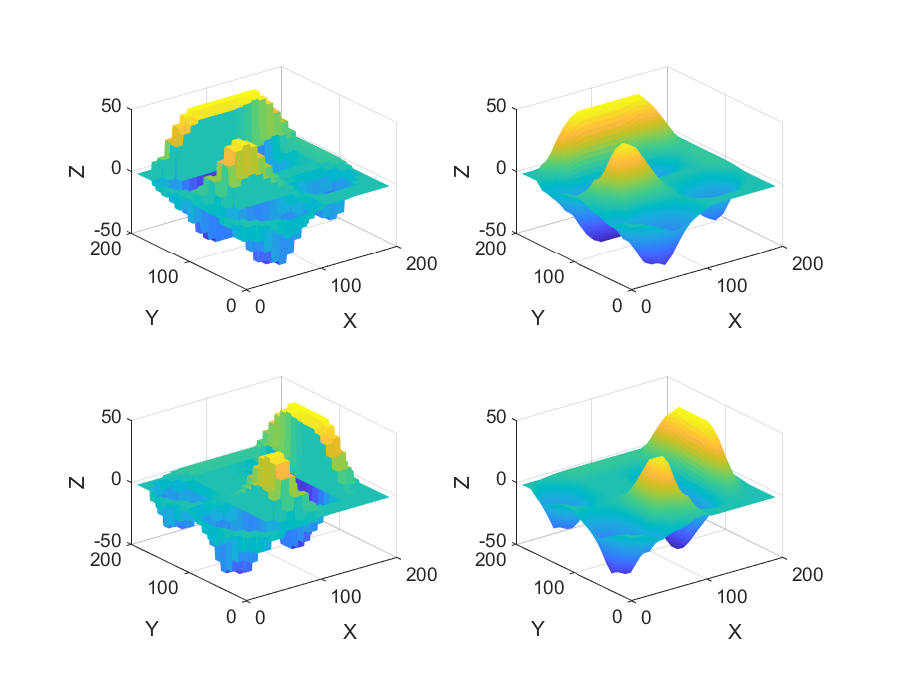
\includegraphics[width=1\linewidth]{non_and_interp_4_plots.eps} % Replace 'example-image' with the filename of your image
	\caption{Repulsive field generation via convolutional kernels. Left: Original repulsive fields in X (top) and Y (bottom) directions. Right: Corresponding fields using interpolation, showcasing enhanced smoothness.}
	\label{fig:interp-experiment}
\end{figure}

\section{MANIPULATOR KINEMATICS}

\subsection{INVERSE KINEMATIC CONTROL}

The desired movement of the end-effector is achieved by using inverse kinematics velocity control scheme with task prioritisation. 

%\begin{equation}
%	\dot{\vec{q}} = J^+ \xi_{p} \mathrm{\vec{v}_{att}} + \dot{\vec{q}}_{rep}
%\end{equation}

\begin{equation}
	\dot{\vec{q}} = \mathbf{J}^+ \xi_{p} \mathrm{\vec{v}{att}} + \dot{\vec{q}}_{rep}
\end{equation}

The damped Moore-Penrose pseudo-inverse, \(\mathbf{J}^+~=~\mathbf{J}'(\mathbf{J}\mathbf{J}' + \sigma_{ee} \mathbf{I})^{-1}\), is utilized to mitigate singularity issues and improve numerical stability in inverse kinematics computations. $\xi_{p}$ is the primary task execution slowdown constant. Finally $\dot{\vec{q}}_{rep}$ are the weighted sum of avoidance joint velocities, each transformed into the null space of primary velocities, as described in the chapter below. 

%\remove{For redundant robots, it optimizes solution selection by minimizing the joint velocity norm, while damping is applied to limit excessive joint velocities near singular configurations, thus improving solution robustness.}

%\add{maybe add the middle joints component in the equation (it is not necessary, doesn't make much change in the chosen experiments)}

We run the inverse kinematics algorithm once for every time step, until we reach the desired cost function or reach the selected time limit. 

\subsection{END-EFFECTOR VELOCITY}

%Vodenje vrha manipulatorja (end-effector) je naloga z najvišjo prioriteto. 

Prioritizing control over the end-effector's (EE) translational velocity is essential for a consistent and stable target approach. The commonly used method, where translational velocity is proportional to squared distance, leads to impractically high initial velocities, which can prevent obstacle avoidance and real-world execution, followed by disproportionately slow velocities when nearing the goal position. Our aim is a consistent velocity profile throughout the trajectory, with controlled deceleration near the goal. This is achieved by first calculating the unit vector towards the target for direction, then modulating its magnitude using a sigmoid function, specifically the arctangent function (eq. \ref{eq: v_att}).

\begin{equation} 
	\vec{v} = \frac{\vec{x}_{EE} - \vec{x}_g}{||\vec{x}_{EE} - \vec{x}_g||} \times \frac{\arctan(k_{sigm} \; ||\vec{x}_{EE} - \vec{x}_g||) }{pi/2}
	\label{eq: v_att}
\end{equation}

%In the above equation (eq.~\ref{eq: v_att}), $\vec{v}$  represents the end effector's translational velocity towards the target, combining direction and magnitude. The terms $\vec{x}_{EE}$ and $\vec{x}_g$ denote the current and goal positions of the EE, respectively, in Cartesian coordinates. The unit vector calculation, $\frac{\vec{x}_{EE}-\vec{x}_g}{||\vec{x}_{EE}-\vec{x}_g||}$, ensures motion directed towards the target. Finally, the sigmoid function, particularly the arctangent component, modulates this velocity to avoid overshooting, balancing speed and precision. The EE velocity will be transformed using the sigmoid curve when near the goal. When the distance from goal point is high, the sigmoid will cause the velocity to get into saturation, that is upper limit. The constant $k_{sigm}$ allows us to set how close to the goal does the robot EE start slowing down and what is the velocity profile when approaching the goal point.


In Eq.~\ref{eq: v_att}, $\vec{v}$ specifies the end-effector's (EE) translational velocity directed towards the target, integrating both its direction and magnitude. Here, $\vec{x}_{EE}$ represents the EE's current position, and $\vec{x}g$ is the target position, both in Cartesian coordinates. The calculation $\frac{\vec{x}{EE}-\vec{x}g}{||\vec{x}{EE}-\vec{x}g||}$ generates a unit vector pointing towards the target, ensuring targeted movement. The velocity's modulation by the arctangent sigmoid function curtails overshooting by moderating speed in proximity to the target and saturating velocity at a predefined upper limit when distant. The parameter \(k_{sigm}\) in the arctangent function adjusts the curve's steepness, affecting how quickly the end-effector decelerates near the target. A higher \(k_{sigm}\) maintains speed until closer to the target for a sharp deceleration, while a lower value starts slowing down earlier for a gradual approach. 

%The rotational error of the EE is needed for ensuring goal orientation of the EE. In our approach, orientations are depicted using rotation matrices. Specifically, \( R \) represents the current EE orientation, while \( gR \) signifies the goal EE orientation. The disparity between these orientations is encapsulated by the relative rotation matrix \( dR \). This matrix is formulated by multiplying the goal orientation matrix \( gR \) with the transpose of the current orientation matrix \( cR^{T} \). To ensure that it represents a pure rotation without any scaling we than normalize the so gotten matrix .

%Determination of the requisite rotation adjustment utilizes the relative rotation matrix \(dR\), calculated from the multiplication of \(gR\) by the \(cR\) transpose, and subsequent normalization to ensure a pure rotational representation. This method guarantees that \(dR\) accurately captures the orientation discrepancy, devoid of any scaling factor.

%The current orientation of the end-effector (EE) and its goal orientation are encoded through rotation matrices, \(cR\) for the current state and \(gR\) for the goal state. The necessary rotational adjustment is identified through the relative rotation matrix \(dR\), generated by multiplying \(gR\) with the transpose of \(cR\) and then normalizing the outcome (eq. \ref{eq: rot_diff_mat}). This process ensures \(dR\) accurately represents rotational differences, without any scaling factors.
%
%To enhance computational efficiency and prevent gimbal lock, the approach transitions from matrix to quaternion representations for precise and efficient rotational velocity adjustments, essential for achieving the target orientation of the EE.

The current orientation of the end-effector (EE) and its goal orientation are encoded through rotation matrices, \(\mathbf{cR}\) for the current state and \(\mathbf{gR}\) for the goal state. The necessary rotational adjustment is identified through the relative rotation matrix \(\mathbf{dR}\), generated by multiplying \(\mathbf{gR}\) with the transpose of \(\mathbf{cR}\) and then normalizing the outcome (eq. \ref{eq: rot_diff_mat}). This process ensures \(\mathbf{dR}\) accurately represents rotational differences, without the effect of any scaling factors.

%\begin{equation}
%	dR = \frac{gR \cdot cR^{T}}{||gR \cdot cR^{T}||}
%	\label{eq: rot_diff_mat}
%\end{equation}

%\begin{equation}
%	\boldsymbol{dR} = \frac{\boldsymbol{gR} \cdot \boldsymbol{cR}^{T}}{\left\lVert\boldsymbol{gR} \cdot \boldsymbol{cR}^{T}\right\rVert}
%	\label{eq: rot_diff_mat}
%\end{equation}

\begin{equation}
	\mathbf{dR} = \frac{\mathbf{gR} \cdot \mathbf{cR}^{T}}{||\mathbf{gR} \cdot \mathbf{cR}^{T}||}
	\label{eq: rot_diff_mat}
\end{equation}

To enhance computational efficiency and prevent gimbal lock, the approach transitions from matrix to quaternion representations for precise and efficient rotational velocity adjustments, essential for achieving the target orientation of the EE.

The relative rotation matrix is converted into a quaternion, which is subsequently logarithmically transformed. The resulting quaternion's components, excluding the real part, constitute the rotational error vector \( \vec{\omega} \).
%
%\begin{equation}
%	dR \mapsto dQ = a + b \, i + c \, j + d \, k
%	\label{eq: quat_mapsto}
%\end{equation}
%
%\begin{equation}
%	dQl = 2 \cdot \log(dQ) = al + bl \, i + cl \, j + dl \, k
%	\label{eq:quat_log}
%\end{equation}

\begin{equation}
	\boldsymbol{dR} \mapsto \boldsymbol{dQ} = a + b \, \vec{i} + c \, \vec{j} + d \, \vec{k}
	\label{eq: quat_mapsto}
\end{equation}

\begin{equation}
	\boldsymbol{dQl} = 2 \cdot \log(\boldsymbol{dQ}) = a_{log} + b_{log} \, \vec{i} + c_{log} \, \vec{j} + d_{log} \, \vec{k}
	\label{eq:quat_log}
\end{equation}

\alert{There needs to be an explanation why log, cite: DMP Quaternions article Žlajpah, Ude}



\begin{equation}
	\vec{\omega} =
	\begin{bmatrix}
		b_{log} \\
		c_{log} \\
		d_{log}
	\end{bmatrix}
	\label{eq:rot_error_vector}
\end{equation}

To get the full velocity of the end effector (EE), \( \mathrm{\vec{v}_{att}} \), we combines translational and rotational velocities, which we scale using proportional gains \( k_v \) and \( k_\omega \).

\begin{equation}
	\mathrm{\vec{v}_{att}} = 
	\begin{bmatrix}
		k_{v} * \vec{v}   \\
		k_{\omega} * \vec{\omega}
	\end{bmatrix}
	\label{eq:ee_velocity}
\end{equation}

%Ker uporabljamo preslikavo v ničelni prostor primarne hitrosti (null space), lahko v primeru velikih hitrosti primarne naloge preostane premalo prostostnih stopenj, da bi se lahko varno izognili oviram. Torej sekundarna naloga izogibanja nima dovolj sposobnosti, prostosti za delovanje.
%
%To ensure the primary task doesn't overpower the secondary task, we've integrated a primary task execution slowdown. This mechanism can reduce the manipulator's velocity towards its primary goal, leaving more maneuverability space for the secondary tasks.
%
%\begin{equation}
%	\label{eq:slowdown}
%	\xi_{p}=
%	\frac{1}{1 + \kappa_{\text{sec}} v_{\text{Rmax}}}
%\end{equation}
%
%The slowdown factor (eq.~\ref{eq:slowdown}) is influenced by the constant \( \kappa_{\text{sec}} \) and the maximum repulsive velocity vectors magnitude, which depends on robot's minimum distance from an obstacle \( v_{\text{Rmax}} \). We calculate the minimal distance in the repulsive velocities phase of the algorithm, as explained in section~\ref{chap:repulsive velocity}. As per the equation, a small \( v_{\text{Rmax}} \) minimizes the slowdown effect, allowing uninterrupted primary task execution. Conversely, a large \( v_{\text{Rmax}} \) increases the slowdown, by making the $\xi_{p}$ factor smaller, giving the secondary task more time for corrective actions.

Utilizing the mapping into the null space of the primary velocity, it becomes evident that at high velocities of the primary task, there may be an insufficient number of degrees of freedom remaining to safely navigate around obstacles. Consequently, the secondary task, which is aimed at obstacle avoidance, lacks the requisite capability and freedom to operate effectively.

\label{chap:primary slowdown}

To mitigate the dominance of the primary task over the secondary task, a mechanism for the deceleration of the primary task's execution has been implemented. This strategy effectively decreases the velocity of the manipulator towards its primary objective, thereby allocating additional maneuverability for secondary tasks.

\begin{equation}
	\label{eq:slowdown}
	\xi_{p}=
	\frac{1}{1 + \kappa_{\text{sec}} ||v_{\text{Rmax}}||}
\end{equation}

The deceleration factor (eq.~\ref{eq:slowdown}) is determined by the constant \( \kappa_{\text{sec}} \) and the magnitude of the maximum repulsive velocity vectors, which is contingent upon the robot's minimal distance from an obstacle \( v_{\text{Rmax}} \). According to the equation, a small \( v_{\text{Rmax}} \) diminishes the deceleration effect, permitting the uninterrupted execution of the primary task. Conversely, large \( v_{\text{Rmax}} \) enhances the deceleration by reducing the $\xi_{p}$ factor, thereby affording the secondary task increased opportunity for obstacles avoidance motion.


\subsection{AVOIDANCE VELOCITIES}

%To move the manipulator away from the obstacles in its environment, we cover the manipulator evenly with virtual detection points (POI). Gostota virtualnih točk je odvisna od velikosti matrik. Če je $w$ širina matrike v smeri pravokotno na primarno smer, je dobro, če so točke medsebojno razmaknjene glede na potek segmentov za $\Delta = \frac{w}{3}$. Tedaj se bodo posamezne matrike deloma pokrivale in dosežemo enakomerno porazdelitev točk (POI) po celotnem robotu. Med izvajanjem kinematične optimizacije izračunavamo izogibne / odbojne hitrosti za vsako od točk po postopku opisanem v zgornjem poglavju. \add{referenca poglavja} To dobimo tako, da izvedemo preslikavo vsake od točk v task space, kjer izvajamo izračun odbojne hitrosti. Pri tem je posamezna kartezična preslikava sestavljena iz kinematične preslikave iz baze robota do začetka segmenta na katerem se točka nahaja in dodane preslikave do izbrane točke (od začetka segmenta do dela kjer se nahaja točka). \(T_{0 \rightarrow \text{POI}} = T_{0 \rightarrow 1} \cdot T_{1 \rightarrow 2} \cdot \ldots \cdot T_{(j-1) \rightarrow j} \cdot T_{j \rightarrow \text{POI}}\) Za vsako od točk dobimo tri komponente kartezične hitrosti. 

To enable the avoidance of obstacles by the manipulator within its operating environment, the manipulator is uniformly coated with virtual detection points (POIs). The density of these virtual points is dependent upon the dimensions of matrices. Given a matrix width $w$ perpendicular to the primary direction, it is advantageous for these points to be spaced at intervals of $\Delta = \frac{w}{3}$. This spacing ensures partial overlap between matrices, thereby achieving a uniform distribution of POIs across the entirety of the robot.

During kinematic optimization, repulsive velocities for each point are computed following the methodology described in the previous section (sect. \ref{section:repulsive_vel}). This is achieved by mapping each point into the task space, where the calculation of repulsive velocity is performed. The cartesian mapping for each point comprises a kinematic transformation from the robot's base to the beginning of the segment where the point is located, followed by an additional mapping to the specific point on the segment (eq. \ref{eq:transformations}).  For each point, three components of cartesian velocity are obtained.

%\begin{equation}
%	T_{0 \rightarrow \text{POI}} = T_{0 \rightarrow 1} \cdot T_{1 \rightarrow 2} \cdot \ldots \cdot T_{(j-1) \rightarrow j} \cdot T_{j \rightarrow \text{POI}}	
%	\label{eq:transformations}
%\end{equation}

\begin{equation}
	\mathbf{T}_{0 \rightarrow \text{POI}} = \mathbf{T}_{0 \rightarrow 1} \cdot \mathbf{T}_{1 \rightarrow 2} \cdot \ldots \cdot \mathbf{T}_{(j-1) \rightarrow j} \cdot \mathbf{T}_{j \rightarrow \text{POI}}	
	\label{eq:transformations}
\end{equation}


%Ko dobimo za vsako od točk odbojno hitrost (repulsive / avoidance velocity), izračunamo drugo normo vsake od hitrosti. Za $K$ točk, v katerih so izogibne hitrosti največje in so posledično najbližje oviri nato izračunamo sklepne hitrosti, ki povzročijo izogibanje oviri. 

Upon obtaining the repulsive velocity for each point, the second norm of each velocity is calculated. For a number of $K$ points where the avoidance velocities are greatest, indicative of closest proximity to an obstacle, the resulting joint velocities that facilitate obstacle avoidance are computed using inverse kinematic equations for the selected points on the manipulator and transformed into the null-space velocities of the primary task.

%\begin{equation}
%J_{d_0}^+ = N J_{d_0}' (J_{d_0} N J_{d_0}' + \sigma_{rep})^{-1};
%\end{equation}

%\begin{equation}
%	J_{d_i}^{+} = N J_{d_i}' (J_{d_i} N J_{d_i}' + \sigma_{rep} I)^{-1}, \quad \text{for } i = 1, 2, \ldots, K;
%\end{equation}

\begin{equation}
	\mathbf{J}_{d_i}^{+} = \mathbf{N} \mathbf{J}_{d_i}' (\mathbf{J}_{d_i} \mathbf{N} \mathbf{J}_{d_i}' + \sigma_{rep} \mathbf{I})^{-1}, \quad \text{for } i = 1, 2, \ldots, K;
\end{equation}


%Za vsako od izbranih točk na robotu izračunamo Jacobijevo transformacijo hitrosti, ki preslika translacijske hitrosti izbrane točke na robotu iz kartezičnega prostora, v prostor sklepov na robotu, ki povezujejo bazo z izbrano točko. V izbranih točkah nas ne zanimajo transformacije napak orientacij. V resnici nas zanima samo komponenta translacijske hitrosti v smeri normale, ki kaže od najbližje točke na objektu proti izbrani točki interesa (POI) na manipulatorju. 

%We calculate translational velocity Jacobian for every of the $K$ selected points on the robot. Since we are only interested in the part of velocity that leads us directly away from the obstacles, we can 

%
%Naš prostor operacij se posledično skrči na eno dimenzijo in the Jacobian, which relates the joint space velocities q and the velocity in the direction of do, can be calculated as  $J_{d_i} = \vec{n}_i^T J_i$.  \add{citat:žlajpah} Pri čemer je vektor normale želene avoidance velocity kar enotski vektor hitrosti, ki ga dobimo s pomočjo naših matrik $\vec{n}_{i} = \frac{\vec{v}_{poi i}}{||\vec{v}_{poi i}||}$. This method offers computational efficiency by eliminating complex matrix inversions, as the Jacobian changes from matrix into a vector dimensions $1 \times n$, where n is number of joints that are located from before the POI and simplifying repulsive velocity calculations.

We calculate the translational velocity Jacobian for each of the $K$ selected points on the robot. Since our interest lies exclusively in the velocity component that directs us away from obstacles, we consequently narrow our operational space to a single dimension. Consequently, the Jacobian, correlating joint space velocities \(q\) with the directional velocity \(d_i\), is represented as \(J_{d_i} = \vec{n}_i^T \mathbf{J}_i\). The normal vector, signifying the desired avoidance velocity, is essentially the unit velocity vector, derived from our matrices as \(\vec{n}_{i} = \frac{\vec{v}_{poi i}}{||\vec{v}_{poi i}||}\). This approach streamlines computational processes by avoiding the necessity for complex matrix inversions, transforming the Jacobian from a matrix to a vector of dimensions \(1 \times n\), where \(n\) signifies the count of joints preceding the POI, thus facilitating more straightforward calculations of repulsive velocities.

\begin{equation}
	\dot{q}_{rep} = k_r \sum_{i=1}^{K} \alpha_i J_{d_i}^{+} \left(v_i - J_{d_i} J^{+} \xi_{p} \vec{v}_{att}\right)
\end{equation}

%Celotne izogibne sklepne hitrosti dobimo z obteženo vsoto izogibnih sklepnih hitrosti izbranih $K$ najbližjih točk, pri čemer upoštevamo vpliv primarne naloge gibanja vrha manipulatorja na sklepne hitrosti.

The overall avoidance joint velocities are obtained through a weighted sum of the avoidance joint velocities for the selected \(K\) nearest points, taking into account the influence of the primary task of manipulator EE movement on the joint velocities.







\section{SIMULATION RESULTS}

\subsection{Repulsive Field Visualization}

%Prvo predstavimo rezultirajoče se odbojno polje za 2D - dvo dimenzijski zemljevid. Načeloma je delovanje na treh dimenzijah enako, seveda pa je to težje vizualizirati. Pri tem smo uporabili našo metodo izračuna odbojnega potencialnega polja hitrosti. Namesto uporabe v točkah robotskem manipulatorju smo točke vzorčili preko celotnega zemljevida ovir, kot je vidno na figur \ref{fig:example-field}. V vsaki od vzorčenih točk smo izvedli v članku opisani postopek pridobivanja odbojnega polja v X in Y smeri. Na spodnjem prikazu figure smo nato vizualizirali odbojno poljo kot vektorsko polje sestavljene iz X in Y komponente.

We introduce the resultant repulsive field on a two-dimensional map. While analogous principles apply to three-dimensional spaces, visualization of more dimensions is complex. Utilizing our repulsive potential field velocity calculation method, points were sampled across the entire obstacle map as depicted in Figure \ref{fig:example-field}. The prescribed algorithm was executed at each sampled point to derive the repulsive fields along the X and Y axes, which were subsequently visualized as a composite vector field.

\begin{figure}
	\centering
	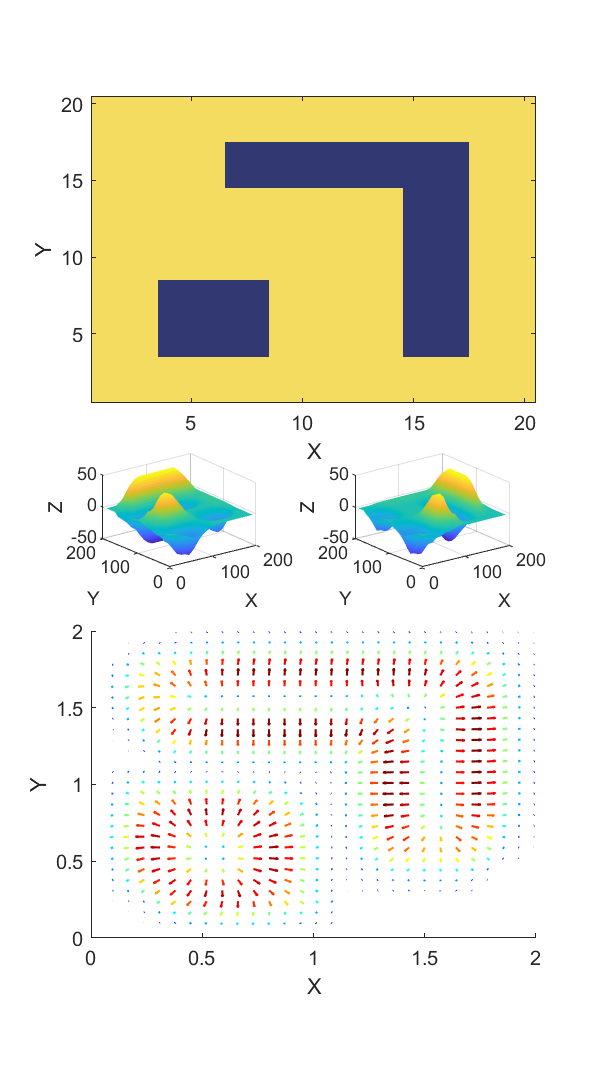
\includegraphics[width=1\linewidth]{demo-field1c.eps} % Replace 'example-image' with the filename of your image
	\caption{Visualization of the potential field calculated for the entire map using the proposed approach. Top: Obstacle distribution via a 2D heatmap. Center: Induced repulsive fields along X (left) and Y (right) axes. Bottom: Composite vector field showcasing the resultant repulsive velocities for obstacle avoidance.}
	\label{fig:example-field}
\end{figure}
%
%\add{add label, caption, every plot has different axis scale}
%
%\comment{}{we dont have the close obstacles bottlenecks, we do have weird bottlenecks in the orthagonal directions - maybe}
%
\subsection{Manipulator Examples}

%Delovanje potencialnega polja smo prikazali na dveh različnih primerih manipulatorja. Pri tem je ločljivost naše mreže voxlov ovir $R=10cm$. Uporaba interpolacije nam omogoča, da imamo relativno grobo mrežo voxlov, kar zniža spominsko zahtevnost mreže prostora, ter pospeši izračun. V primerih smo izbrali $K = 7$ POI točk interesa, v katerih gledamo oddaljenost od ovir, ki so enakomerno razporejene po segmentih in sklepih od drugega sklepa robota do vrha manipulatorja, torej od prve točke naprej, kjer se je manipulator sposoben izogniti oviri. POI so na grafih prikazani s pikami na manipulatorju. V bližini ovir iz njih segajo vektorji, ki prikazujejo izračunane odbojno hitrost v točkah. 

%Med izvajanjem simulacije izvajamo eulerjevo integracijo izračunanih sklepnih hitrosti, s korakom $T_{step}=0.1s$.

The operation of the potential field is demonstrated on two different manipulator cases. The resolution of our voxel grid for obstacles is \( R=10cm \). The use of interpolation allows us to have a relatively coarse voxel grid, which reduces the memory demand of the space grid and accelerates the computation. We selected \( K = 7 \) Points of Interest (POI) to observe the distance from obstacles and are uniformly distributed them along the segments and joints, starting from the second joint of the robot to the tip of the manipulator. This distribution begins from the second joint because it is from this point onwards that the manipulator has the capability to avoid obstacles. Points of Interest (POIs) are indicated by dots on the manipulator in the graphs. Near obstacles, vectors emanate from these points, depicting the calculated repulsive velocities at the locations. Throughout the simulation, Euler integration of the calculated joint velocities is performed with a step size of \( T_{step} = 0.1 \) s.

%V prvem primeru \ref{fig:keyframes-3d-column} manipulator z uporabo potencialnega polja izračunanega na predlagani način, se manipulator varno "zvije" oziroma izbere pot do točke, ki se nahaja na drugi strani stebra. Izbrane konstante primarne naloge so $k_v=5$ in $k_w=20$. Izbrane konstante obteženosti posameznih POI so $\alpha=\frac{\left[ \frac{3}{9}, \frac{2}{9}, \frac{1}{9}, \frac{1}{9}, \frac{1}{9}, \frac{1}{9}
% \right]}{10}$. Najkrajša pot vrha v točko pelje direktno skozi steber. Primarna naloga je, da vrh preide v želeno pozicijo in orientacijo. Ker je naloga vrha primarna, moramo uvesti znižanje primarne hitrosti v bližini ovire $\xi_{p}=1$, da ima sekundarna naloga dovolj prostosti in časa, da lahko izvede rekonfiguracijo za obhod stebra. Simulacijo izvajamo $50$ korakov. 

In the first case (Fig. \ref{fig:keyframes-3d-column}, \ref{fig:plots-3d-column}), the manipulator safely 'curls' or selects a path to a point located on the other side of a column, avoiding the obstacle with the potential field calculated by the proposed method. The constants chosen for the primary task are \( k_v = 5 \) and \( k_w = 1.5 \), for the avoidance task \(k_r=20\). The weighting constants for the individual POIs are \( \alpha = \frac{[ \frac{3}{9}, \frac{2}{9}, \frac{1}{9}, \frac{1}{9}, \frac{1}{9}, \frac{1}{9} ]}{10} \), where the biggest weight belongs to the point on the manipulator which is closest to the obstacle and so on. As the most direct path for the end-effector to the target passes straight through the column, an approach that would result in a collision, we implement a reduction of the primary speed in the vicinity of the obstacle, setting \( \xi_{p} = 1 \). The simulation is performed for 50 steps. 

\begin{figure}
	\centering
	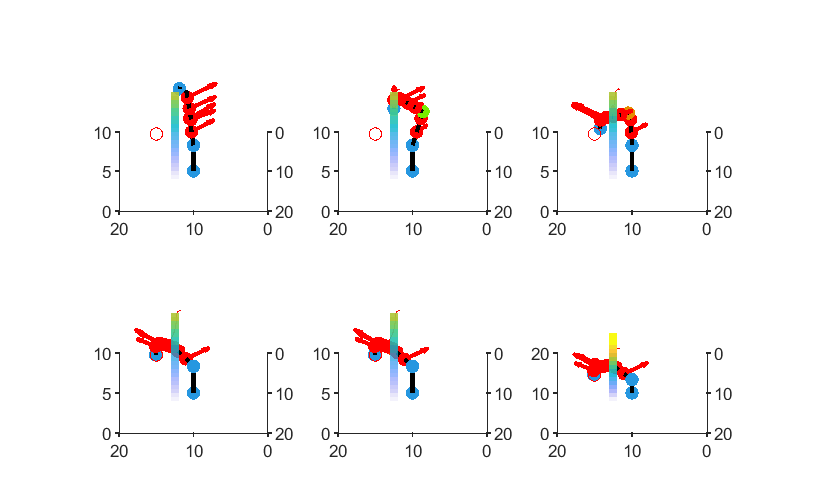
\includegraphics[width=1\linewidth]{keyframes_3D.eps} % Replace 'example-image' with the filename of your image
	\caption{Sequential keyframes demonstrating the manipulator's path planning and column obstacle avoidance strategy.}
	\label{fig:keyframes-3d-column}
\end{figure}


\begin{figure}
	\centering
	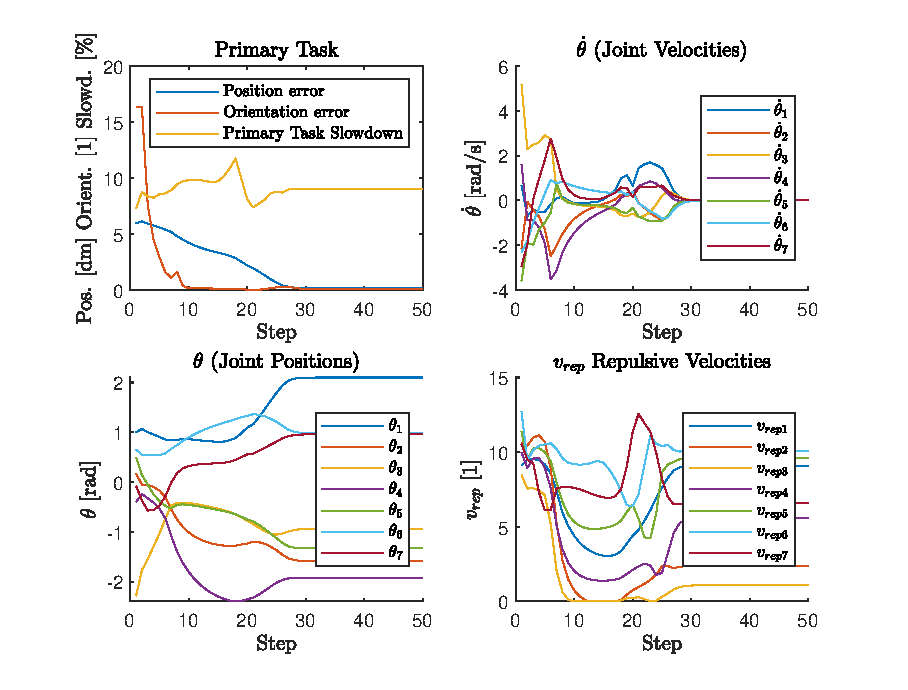
\includegraphics[width=1\linewidth]{4plots_column.eps} % Replace 'example-image' with the filename of your image
	\caption{Visualization of the manipulator's path around the column obstacle: (a) Primary Task errors and percentage of the primary speed after applying slowdown, (b) Joint Velocities $\dot{\theta}$, (c) Joint Positions $\theta$, and (d) Norms of Repulsive Velocities $v_{rep}$.}
	\label{fig:plots-3d-column}
\end{figure}

%V drugem primeru (Fig. \ref{fig:keyframes-3d-ball}, \ref{fig:plots-ball}) se naš robot giblje v dinamične okolju. Predlagan način izračuna odbojnih hitrosti je dobra izbira v primeru, ko potrebujemo lokalno optimizacijsko metodo za upoštevanje dinamičnih spremeb. V izbranem primeru imamo žogo, ki se med potekom optimizacije enakomerno premika iz leve strani grafa proti desni strani (torej v smeri y osi od 0.4 v trenutku 0 do 1.4 v zadnjem koraku simulacije). Primarna naloga ima sedaj nalogo vzdrževati vrh robota v eni točki, pri čemer smo za večjo sposobnost izogibanja oviri zanemarili izbiro orientacije vrha EE. To nam poveča sposobnost gibanja, posledično ne potrebujemo primary speed task slowdown  \( \xi_{p} = 0 \). The constants chosen for the primary task are \( k_v = 2 \) and \( k_w = 0 \), for the avoidance task \(k_r=3\). The weighting constants for the individual POIs are \( \alpha = \frac{[ \frac{1}{5}, \frac{1}{5}, \frac{1}{5}, \frac{1}{5}, \frac{1}{5}, \frac{1}{5} ]}{10} \). 

In the second scenario (Fig. \ref{fig:keyframes-3d-ball}, \ref{fig:plots-ball}), our robot operates within a dynamic environment. The proposed method for calculating repulsive velocities proves to be a suitable choice when a local optimization approach is needed to accommodate dynamic changes. In this scenario, a ball moves consistently from the left to the right side of the graph (i.e., along the y-axis from 0.4 at the initial moment to 1.4 in the final step of the simulation), as governed by the equation \( y_{\text{ball}} = 0.4 + (1.4 - 0.4) \times \frac{N_{\text{step}}}{75} \),  with \( x_{\text{ball}} = 1.25 \) and \( z_{\text{ball}} = 0.7 \). The primary task is now to maintain the robot's end-effector (EE) at a fixed point, disregarding EE orientation to enhance obstacle avoidance capability. This increases maneuverability, thereby eliminating the need for primary speed task slowdown (\( \xi_{p} = 0 \)). Constants selected for the primary task are \( k_v = 2 \) and \( k_w = 0 \), and for the avoidance task \( k_r = 3 \). Weighting constants for the individual POIs are \( \alpha = \frac{[ \frac{1}{5}, \frac{1}{5}, \frac{1}{5}, \frac{1}{5}, \frac{1}{5}, \frac{1}{5} ]}{10} \). The simulation is performed for 75 steps. 

\add{describe weights and distributions used in the kernels}

\add{sigmoid weights}

%\begin{figure}
%	\centering
%	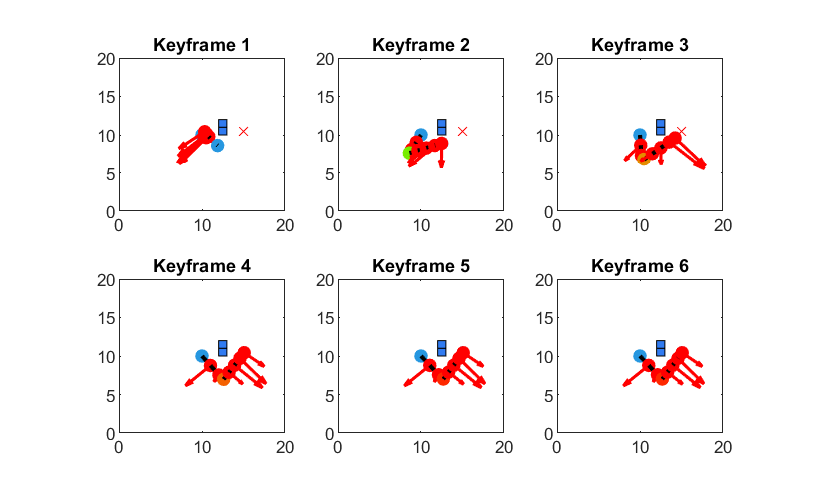
\includegraphics[width=1\linewidth]{keyframes_2D_a.eps} % Replace 'example-image' with the filename of your image
%	\caption{Example Image}
%	\label{fig:keyframes-2d-column}
%\end{figure}
%
%\begin{figure}
%	\centering
%	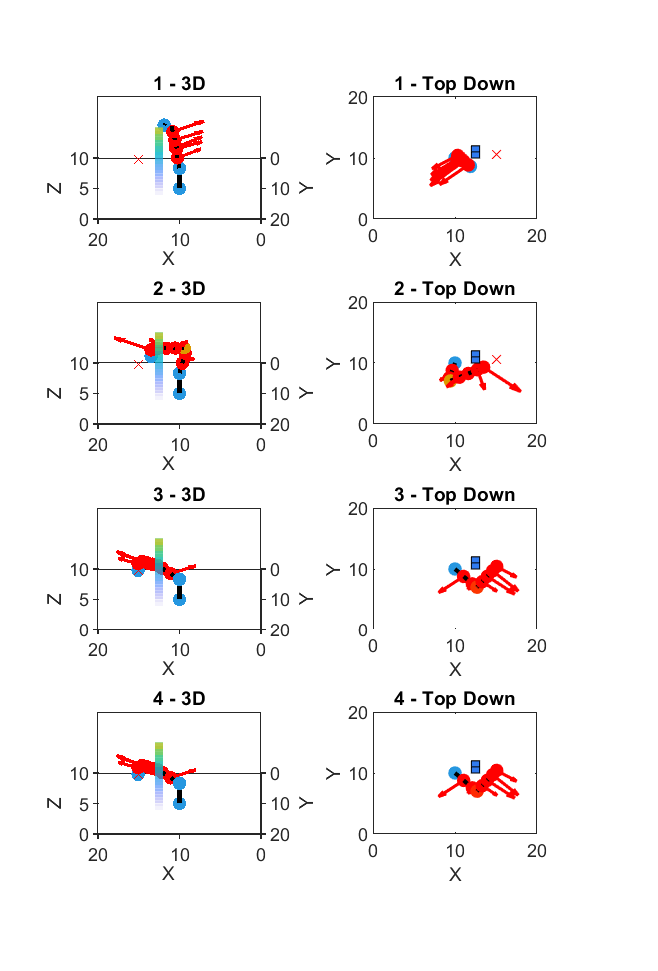
\includegraphics[width=1\linewidth]{keyframes_2_columns.eps} % Replace 'example-image' with the filename of your image
%	\caption{Example Image}
%	\label{fig:keyframes-2-column}
%\end{figure}
%
%
%\add{EXAMPLE: MANIPULATOR AND MOVING NOISY BALL}
%
\begin{figure}
	\centering
	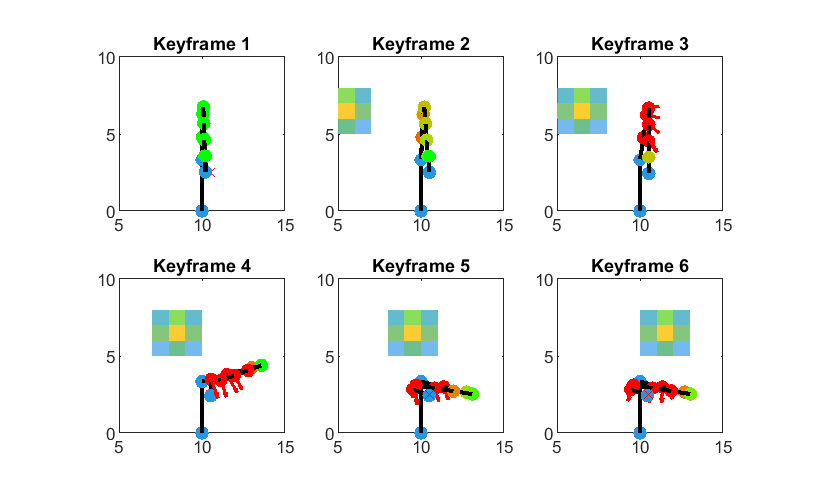
\includegraphics[width=1\linewidth]{keyframes_2D_ball.eps} % Replace 'example-image' with the filename of your image
	\caption{Dynamic obstacle avoidance scenario: Sequential keyframes illustrating the robot’s maneuvering in response to a progressively moving ball from left to right across the workspace.}
	\label{fig:keyframes-3d-ball}
\end{figure}
%
%\begin{figure}
%	\centering
%	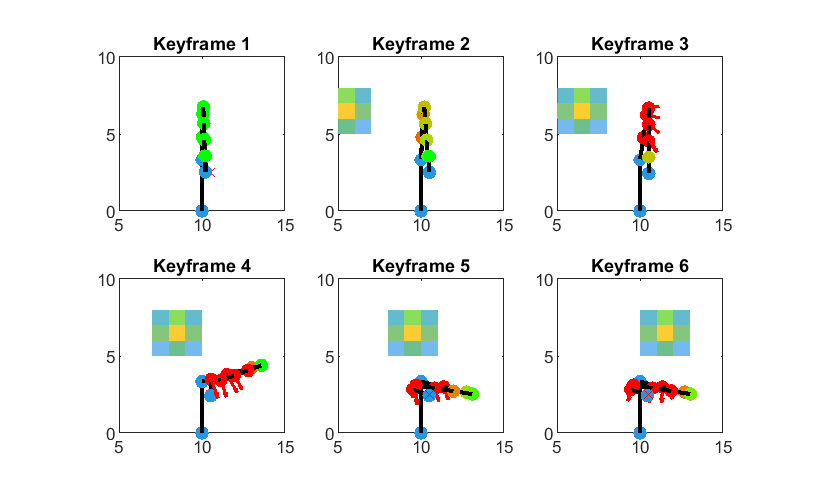
\includegraphics[width=1\linewidth]{keyframes_2D_ball.eps} % Replace 'example-image' with the filename of your image
%	\caption{Example Image}
%	\label{fig:keyframes-2d-ball}
%\end{figure}
%
\begin{figure}
	\centering
	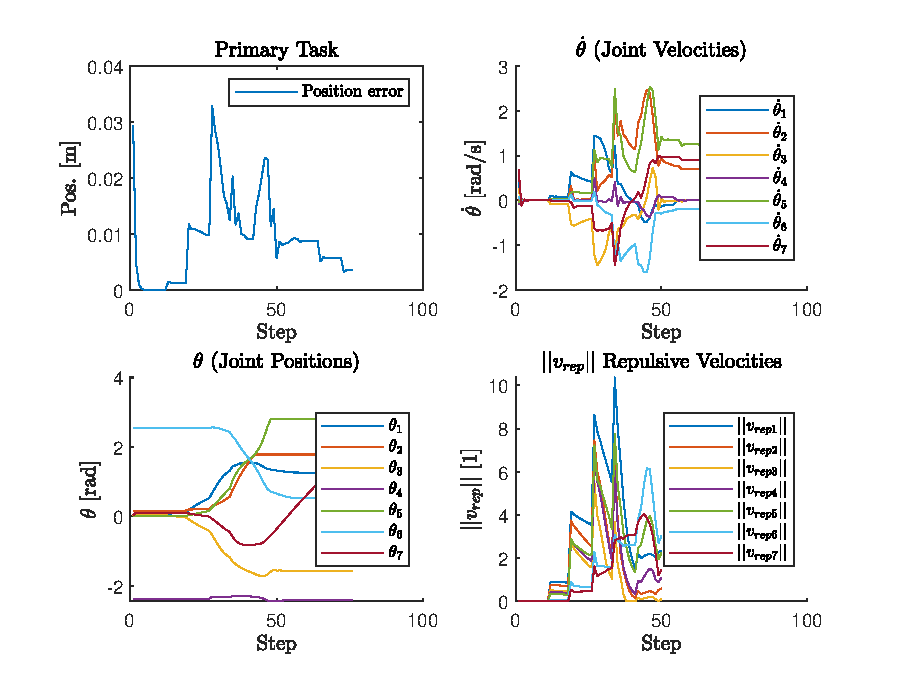
\includegraphics[width=1\linewidth]{4plots_ball.eps} % Replace 'example-image' with the filename of your image
	\caption{Performance in a dynamic obstacle avoidance scenario: (a) Primary Task error (b) Joint Velocities $\dot{\theta}$, (c) Joint Positions $\theta$, and (d) Norms of Repulsive Velocities $v_{rep}$.}
	\label{fig:plots-ball}
\end{figure}
%



\section{CONCLUSION}

\add{ADD}

\addtolength{\textheight}{-12cm}   % This command serves to balance the column lengths
                                  % on the last page of the document manually. It shortens
                                  % the textheight of the last page by a suitable amount.
                                  % This command does not take effect until the next page
                                  % so it should come on the page before the last. Make
                                  % sure that you do not shorten the textheight too much.


\begin{thebibliography}{99}
	
\bibitem{siciliano1990kinematic} B. Siciliano, “Kinematic control of redundant robot manipulators: A tutorial,” J. Intell. Robot. Syst., vol. 3, no. 3, Art. no. 3, 1990, doi: 10.1007/BF00126069.

\bibitem{siciliano2010robot} B. Siciliano, L. Sciavicco, L. Villani, and G. Oriolo, Robot. Model. Plan. Control, 2010, pp. 161–189. [Online]. Available: http://link.springer.com/10.1007/978-1-84628-642-1\_4

%\bibitem{vsvestka1997motion} P. {\v{S}}vestka and M. H. Overmars, “Motion planning for carlike robots using a probabilistic learning approach,” The International Journal of Robotics Research, vol. 16, no. 2, pp. 119–143, 1997.

\bibitem{lavalle1998rapidly} S. LaValle, “Rapidly-exploring random trees: A new tool for path planning,” Research Report 9811, 1998.

\bibitem{gammell2015batch} J. D. Gammell, S. S. Srinivasa, and T. D. Barfoot, “Batch Informed Trees (BIT*): Sampling-based Optimal Planning via the Heuristically Guided Search of Implicit Random Geometric Graphs,” in Proc. of the 2015 IEEE International Conference on Robotics and Automation (ICRA), May 2015, pp. 3067–3074. doi: 10.1109/ICRA.2015.7139620.

\bibitem{karaman2010incremental} S. Karaman and E. Frazzoli, "Incremental sampling-based algorithms for optimal motion planning," in Proc. Robotics: Science and Systems (RSS), 2010.

\bibitem{kuffner2000rrt} J. J. Kuffner and S. M. LaValle, “RRT-connect: An efficient approach to single-query path planning,” in Proceedings of the 2000 ICRA. Millennium Conference. IEEE International Conference on Robotics and Automation. Symposia Proceedings (Cat. No.00CH37065), Apr. 2000, pp. 995–1001 vol.2. doi: 10.1109/ROBOT.2000.844730.

\bibitem{c29} A. A. Maciejewski and C. A. Klein, “Obstacle Avoidance for Kinematically Redundant Manipulators in Dynamically Varying Environments,” The International Journal of Robotics Research, vol. 4, no. 3, pp. 109–117, Sep. 1985. doi: 10.1177/027836498500400308.

\bibitem{c38} Y. Nakamura, H. Hanafusa, and T. Yoshikawa, “Task-Priority Based Redundancy Control of Robot Manipulators,” The International Journal of Robotics Research, vol. 6, no. 2, pp. 3–15, Jun. 1987. doi: 10.1177/027836498700600201.

\bibitem{c21} E. A. Basso and K. Y. Pettersen, “Task-Priority Control of Redundant Robotic Systems using Control Lyapunov and Control Barrier Function based Quadratic Programs,” in IFAC-PapersOnLine, vol. 53, no. 2, pp. 9037–9044, 2020. doi: 10.1016/j.ifacol.2020.12.2024.

\bibitem{c23} H. Toshani and M. Farrokhi, “Real-time inverse kinematics of redundant manipulators using neural networks and quadratic programming: A Lyapunov-based approach,” Robotics and Autonomous Systems, vol. 62, no. 6, pp. 766–781, Jun. 2014. doi: 10.1016/j.robot.2014.02.005.

%\bibitem{c22} Y. Zhang, S. S. Ge, and T. H. Lee, “A Unified Quadratic-Programming-Based Dynamical System Approach to Joint Torque Optimization of Physically Constrained Redundant Manipulators,” IEEE Trans. Syst., Man, Cybern. B, vol. 34, no. 5, pp. 2126–2132, Oct. 2004. doi: 10.1109/TSMCB.2004.830347.

\bibitem{c44} Z. Long, “Virtual target point-based obstacle-avoidance method for manipulator systems in a cluttered environment,” Engineering Optimization, vol. 52, no. 11, Art. no. 11, Nov. 2020. doi: 10.1080/0305215X.2019.1681986.

\bibitem{c33} O. Khatib, “Real-time obstacle avoidance for manipulators and mobile robots,” in 1985 IEEE International Conference on Robotics and Automation Proceedings, Mar. 1985, pp. 500–505. doi: 10.1109/ROBOT.1985.1087247.

%\bibitem{c40} J.-O. Kim and P. Khosla, “Real-Time Obstacle Avoidance Using Harmonic Potential Functions,” 1992. doi: 10.1109/70.143352.

\bibitem{c43} M. F. Pinto, T. R. F. Mendonça, L. R. Olivi, E. B. Costa, and A. L. M. Marcato, “Modified approach using variable charges to solve inherent limitations of potential fields method,” in Proc. 2014 11th IEEE/IAS International Conference on Industry Applications, Dec. 2014, pp. 1–6. doi: 10.1109/INDUSCON.2014.7059414.

\bibitem{c45} A. H. Qureshi and Y. Ayaz, “Potential Functions based Sampling Heuristic For Optimal Path Planning,” Auton Robot, vol. 40, no. 6, Art. no. 6, Aug. 2016. doi: 10.1007/s10514-015-9518-0.

%\bibitem{c46} A. H. Qureshi et al., “Adaptive Potential guided directional-RRT*,” in Proc. 2013 IEEE International Conference on Robotics and Biomimetics (ROBIO), Shenzhen, China, Dec. 2013, pp. 1887–1892. doi: 10.1109/ROBIO.2013.6739744.

\bibitem{c47} J. Yi, Q. Yuan, R. Sun, and H. Bai, “Path planning of a manipulator based on an improved P\_RRT* algorithm,” Complex Intell. Syst., vol. 8, no. 3, pp. 2227–2245, Jun. 2022. doi: 10.1007/s40747-021-00628-y.

\bibitem{klancar2022robot}
G. Klančar, A. Zdešar, and M. Krishnan, “Robot Navigation Based on Potential Field and Gradient Obtained by Bilinear Interpolation and a Grid-Based Search,” Sensors, vol. 22, no. 9, art. no. 3295, pp. 1-24, 2022. doi: 10.3390/s22093295.

\bibitem{c49} X. Xia et al., “Path Planning for Obstacle Avoidance of Robot Arm Based on Improved Potential Field Method,” Sensors, vol. 23, no. 7, Art. no. 7, Apr. 2023. doi: 10.3390/s23073754.

\bibitem{park2020trajectory} S.-O. Park, M. C. Lee, and J. Kim, “Trajectory Planning with Collision Avoidance for Redundant Robots Using Jacobian and Artificial Potential Field-based Real-time Inverse Kinematics,” Int. J. Control Autom. Syst., vol. 18, no. 8, Art. no. 8, Aug. 2020, doi: 10.1007/s12555-019-0076-7.

\bibitem{baumgartner2023potential}
J. Baumgartner, T. Petrič, and G. Klančar, “Potential Field Control of a Redundant Nonholonomic Mobile Manipulator with Corridor-Constrained Base Motion,” Machines, vol. 11, no. 2, art. no. 293, pp. 1-28, 2023. doi: 10.3390/machines11020293.

\bibitem{oleynikova2017voxblox} H. Oleynikova, Z. Taylor, M. Fehr, R. Siegwart, and J. Nieto, “Voxblox: Incremental 3D Euclidean Signed Distance Fields for on-board MAV planning,” in Proc. of the 2017 IEEE/RSJ International Conference on Intelligent Robots and Systems (IROS), Vancouver, BC, Sep. 2017, pp. 1366–1373. doi: 10.1109/IROS.2017.8202315.

\bibitem{han2019fiesta} L. Han, F. Gao, B. Zhou, and S. Shen, “FIESTA: Fast Incremental Euclidean Distance Fields for Online Motion Planning of Aerial Robots,” arXiv, Jul. 26, 2019. Accessed: Jan. 11, 2024. [Online]. Available: http://arxiv.org/abs/1903.02144

\bibitem{lau2010improved} B. Lau, C. Sprunk, and W. Burgard, “Improved updating of Euclidean distance maps and Voronoi diagrams,” in Proc. of the 2010 IEEE/RSJ International Conference on Intelligent Robots and Systems, Taipei, Oct. 2010, pp. 281–286. doi: 10.1109/IROS.2010.5650794.

\bibitem{rong2006jump} G. Rong and T.-S. Tan, “Jump flooding in GPU with applications to Voronoi diagram and distance transform,” in Proceedings of the 2006 Symposium on Interactive 3D Graphics and Games - SI3D ’06, Redwood City, California, 2006, p. 109. doi: 10.1145/1111411.1111431.

\bibitem{zhou2021egoplanner} X. Zhou, Z. Wang, H. Ye, C. Xu, and F. Gao, “EGO-Planner: An ESDF-Free Gradient-Based Local Planner for Quadrotors,” IEEE Robot. Autom. Lett., vol. 6, no. 2, pp. 478–485, Apr. 2021, doi: 10.1109/LRA.2020.3047728.







%\bibitem{gammell2014informed} J. D. Gammell, S. S. Srinivasa, and T. D. Barfoot, “Informed RRT*: Optimal sampling-based path planning focused via direct sampling of an admissible ellipsoidal heuristic,” in Proc. of the 2014 IEEE/RSJ International Conference on Intelligent Robots and Systems, Chicago, IL, USA, Sep. 2014, pp. 2997–3004. doi: 10.1109/IROS.2014.6942976.
%
%	
%\bibitem{IDEASLab2023}
%IDEAS Lab, "Motion and Path Planning," presented at Purdue University, 2023. [Online]. Available: \url{https://ideas.cs.purdue.edu/research/robotics/planning/}. Accessed on: Jan. 9, 2024.
%	





\bibitem{haviland2021neo} J. Haviland and P. Corke, “NEO: A Novel Expeditious Optimisation Algorithm for Reactive Motion Control of Manipulators,” IEEE Robot. Autom. Lett., vol. 6, no. 2, Art. no. 2, Apr. 2021, doi: 10.1109/LRA.2021.3056060.




\bibitem{c24} J. Nakanishi, R. Cory, M. Mistry, J. Peters, and S. Schaal, “Comparative experiments on task space control with redundancy resolution,” in Proc. 2005 IEEE/RSJ Int. Conf. on Intelligent Robots and Systems, Edmonton, Alta., Canada, 2005, pp. 3901–3908. doi: 10.1109/IROS.2005.1545203.

\bibitem{c25} M. H. Raibert and J. J. Craig, “Hybrid Position/Force Control of Manipulators,” Journal of Dynamic Systems, Measurement, and Control, vol. 103, no. 2, pp. 126–133, Jun. 1981. doi: 10.1115/1.3139652.

\bibitem{c26} T. Yoshikawa, “Dynamic hybrid position/force control of robot manipulators--Description of hand constraints and calculation of joint driving force,” IEEE J. Robot. Automat., vol. 3, no. 5, pp. 386–392, Oct. 1987. doi: 10.1109/JRA.1987.1087120.

\bibitem{c27} O. Khatib, “A unified approach for motion and force control of robot manipulators: The operational space formulation,” IEEE J. Robot. Automat., vol. 3, no. 1, pp. 43–53, Feb. 1987. doi: 10.1109/JRA.1987.1087068.

\bibitem{c28} N. Hogan, “Impedance Control: An Approach to Manipulation,” in Proc. 1984 American Control Conf., San Diego, CA, USA, Jul. 1984, pp. 304–313. doi: 10.23919/ACC.1984.4788393.



\bibitem{c30} L. Lajpah and T. Petri, “Obstacle Avoidance for Redundant Manipulators as Control Problem,” in Serial and Parallel Robot Manipulators - Kinematics, Dynamics, Control and Optimization, S. Kucuk, Ed. InTech, 2012. doi: 10.5772/32651.

\bibitem{c31} R. Colbaugh and K. Glass, “Cartesian control of redundant robots,” J. Robotic Syst., vol. 6, no. 4, pp. 427–459, Aug. 1989. doi: 10.1002/rob.4620060409.

\bibitem{c32} K. Glass, R. Colbaugh, D. Lim, and H. Seraji, “Real-time collision avoidance for redundant manipulators,” IEEE Trans. Robot. Automat., vol. 11, no. 3, pp. 448–457, Jun. 1995. doi: 10.1109/70.388789.



\bibitem{c34} L. Sciavicco and B. Siciliano, “A solution algorithm to the inverse kinematic problem for redundant manipulators,” IEEE J. Robot. Automat., vol. 4, no. 4, pp. 403–410, Aug. 1988. doi: 10.1109/56.804.

\bibitem{c35} L. Sciavicco and B. Siciliano, “Solving the Inverse Kinematic Problem for Robotic Manipulators,” in RoManSy 6, A. Morecki, G. Bianchi, and K. Kedzior, Eds., Boston, MA: Springer US, 1987, pp. 107–114. doi: 10.1007/978-1-4684-6915-8\_9.

\bibitem{c36} O. Egeland, “Task-space tracking with redundant manipulators,” IEEE J. Robot. Automat., vol. 3, no. 5, pp. 471–475, Oct. 1987. doi: 10.1109/JRA.1987.1087118.

\bibitem{c37} H. Seraji, “Configuration control of redundant manipulators: theory and implementation,” IEEE Trans. Robot. Automat., vol. 5, no. 4, pp. 472–490, Aug. 1989. doi: 10.1109/70.88062.



\bibitem{c39} B. Siciliano and O. Khatib, Eds., Springer Handbook of Robotics. in Springer Handbooks. Cham: Springer International Publishing, 2016. doi: 10.1007/978-3-319-32552-1.



\bibitem{c41} L. Zlajpah and B. Nemec, “Kinematic control algorithms for on-line obstacle avoidance for redundant manipulators,” in Proc. IEEE/RSJ International Conference on Intelligent Robots and Systems, Lausanne, Switzerland, 2002, pp. 1898–1903. doi: 10.1109/IRDS.2002.1044033.

\bibitem{c42} T. Petrič and L. Žlajpah, “Smooth continuous transition between tasks on a kinematic control level: Obstacle avoidance as a control problem,” Robotics and Autonomous Systems, vol. 61, no. 9, Art. no. 9, Sep. 2013. doi: 10.1016/j.robot.2013.04.019.







\bibitem{c48} T. Zhu, J. Mao, L. Han, C. Zhang, and J. Yang, “Real-Time Dynamic Obstacle Avoidance for Robot Manipulators Based on Cascaded Nonlinear MPC With Artificial Potential Field,” IEEE Trans. Ind. Electron., pp. 1–11, 2023. doi: 10.1109/TIE.2023.3306405.



\bibitem{c50} Y. Chen, L. Chen, J. Ding, and Y. Liu, “Research on Real-Time Obstacle Avoidance Motion Planning of Industrial Robotic Arm Based on Artificial Potential Field Method in Joint Space,” Applied Sciences, vol. 13, no. 12, p. 6973, Jan. 2023. doi: 10.3390/app13126973.

\bibitem{c51} S. M. LaValle, Planning Algorithms. Cambridge: Cambridge University Press, 2006.

\bibitem{c52} M. G. Tamizi, M. Yaghoubi, and H. Najjaran, “A review of recent trend in motion planning of industrial robots,” Int J Intell Robot Appl, vol. 7, no. 2, Art. no. 2, Jun. 2023. doi: 10.1007/s41315-023-00274-2.







\bibitem{siciliano2016springer} B. Siciliano and O. Khatib, Eds., Springer Handbook of Robotics, in Springer Handbooks. Cham: Springer International Publishing, 2016. doi: 10.1007/978-3-319-32552-1.



\bibitem{dai2022review} Y. Dai, C. Xiang, Y. Zhang, Y. Jiang, W. Qu, and Q. Zhang, “A Review of Spatial Robotic Arm Trajectory Planning,” Aerospace, vol. 9, p. 361, Jul. 2022, doi: 10.3390/aerospace9070361.

\bibitem{gottschalk1996obbtree} S. Gottschalk, M. C. Lin, and D. Manocha, “OBBTree: a hierarchical structure for rapid interference detection,” in Proceedings of the 23rd Annual Conference on Computer Graphics and Interactive Techniques, ACM, Aug. 1996, pp. 171–180. doi: 10.1145/237170.237244.

\bibitem{vandenbergen1997efficient} G. van den Bergen, “Efficient Collision Detection of Complex Deformable Models using AABB Trees,” Journal of Graphics Tools, vol. 2, no. 4, pp. 1–13, 1997. doi: 10.1080/10867651.1997.10487480.

\bibitem{chen2018path} G. Chen, D. Liu, Y. Wang, Q. Jia, and X. Zhang, “Path planning method with obstacle avoidance for manipulators in dynamic environment,” International Journal of Advanced Robotic Systems, vol. 15, no. 6, Art. no. 1729881418820223, Nov. 2018, doi: 10.1177/1729881418820223.

\bibitem{puiu2011realtime} D. Puiu and F. Moldoveanu, “Real-time collision avoidance for redundant manipulators,” in Proc. of the 2011 6th IEEE International Symposium on Applied Computational Intelligence and Informatics (SACI), Timisoara, Romania, 2011, pp. 403–408, doi: 10.1109/SACI.2011.5873037.



\bibitem{wurmOctoMap} K. M. Wurm, A. Hornung, M. Bennewitz, C. Stachniss, and W. Burgard, “OctoMap: A Probabilistic, Flexible, and Compact 3D Map Representation for Robotic Systems,” [Details of publication, e.g., in Proc. of the Conference/Journal Name, Year, pp. Page numbers]. [DOI or URL if available].

\bibitem{gao2019flying} F. Gao, W. Wu, W. Gao, and S. Shen, “Flying on point clouds: Online trajectory generation and autonomous navigation for quadrotors in cluttered environments,” Journal of Field Robotics, vol. 36, no. 4, pp. 710–733, 2019, doi: 10.1002/rob.21842.

\bibitem{elfes1989using} A. Elfes, “Using occupancy grids for mobile robot perception and navigation,” Computer, vol. 22, no. 6, pp. 46–57, Jun. 1989, doi: 10.1109/2.30720.



\bibitem{xu2021voxel} Y. Xu, X. Tong, and U. Stilla, “Voxel-based representation of 3D point clouds: Methods, applications, and its potential use in the construction industry,” Automation in Construction, vol. 126, p. 103675, Jun. 2021, doi: 10.1016/j.autcon.2021.103675.

\bibitem{niessner2013realtime} M. Nießner, M. Zollhöfer, S. Izadi, and M. Stamminger, “Real-time 3D reconstruction at scale using voxel hashing,” ACM Trans. Graph., vol. 32, no. 6, pp. 1–11, Nov. 2013, doi: 10.1145/2508363.2508374.

\bibitem{dryanovski2010multivolume} I. Dryanovski, W. Morris, and J. Xiao, “Multi-volume occupancy grids: An efficient probabilistic 3D mapping model for micro aerial vehicles,” in Proc. of the 2010 IEEE/RSJ International Conference on Intelligent Robots and Systems, Taipei, Oct. 2010, pp. 1553–1559. doi: 10.1109/IROS.2010.5652494.

\bibitem{thrun2002probabilistic} S. Thrun, Probabilistic robotics, vol. 45, 2002. Accessed: Jun. 14, 2023. [Online]. Available: https://dl.acm.org/doi/10.1145/504729.504754



\bibitem{luo2018collisionfree} L. Luo et al., “Collision-Free Path-Planning for Six-DOF Serial Harvesting Robot Based on Energy Optimal and Artificial Potential Field,” Complexity, vol. 2018, pp. 1–12, Nov. 2018, doi: 10.1155/2018/3563846.

\bibitem{zhang2021obstacle} W. Zhang, H. Cheng, L. Hao, X. Li, M. Liu, and X. Gao, “An obstacle avoidance algorithm for robot manipulators based on decision-making force,” Robotics and Computer-Integrated Manufacturing, vol. 71, p. 102114, Oct. 2021, doi: 10.1016/j.rcim.2020.102114.



\bibitem{han2018dynamic} D. Han, H. Nie, J. Chen, and M. Chen, “Dynamic obstacle avoidance for manipulators using distance calculation and discrete detection,” Robotics and Computer-Integrated Manufacturing, vol. 49, pp. 98–104, Feb. 2018, doi: 10.1016/j.rcim.2017.05.013.



\bibitem{szeliski2021computer} R. Szeliski, “Computer Vision: Algorithms and Applications, 2nd Edition,” Springer, 2021.

\bibitem{rosenfeld1968distance} A. Rosenfeld and J. L. Pfaltz, “Distance functions on digital pictures,” Pattern Recognition, vol. 1, no. 1, pp. 33–61, Jul. 1968, doi: 10.1016/0031-3203(68)90013-7.

\bibitem{felzenszwalb2012distance} P. F. Felzenszwalb and D. P. Huttenlocher, “Distance Transforms of Sampled Functions,” Theory of Comput., vol. 8, no. 1, pp. 415–428, 2012, doi: 10.4086/toc.2012.v008a019.



\bibitem{dryanovski2010multivolume} I. Dryanovski, W. Morris, and J. Xiao, “Multi-volume occupancy grids: An efficient probabilistic 3D mapping model for micro aerial vehicles,” in 2010 IEEE/RSJ International Conference on Intelligent Robots and Systems, Taipei: IEEE, Oct. 2010, pp. 1553–1559, doi: 10.1109/IROS.2010.5652494.



\end{thebibliography}




\end{document}
